\documentclass[12pt]{article}

\usepackage[utf8x]{inputenc}
\usepackage[spanish,es-noshorthands]{babel}

\usepackage{amssymb,amsmath,amsthm,amsfonts}
\usepackage{calc}
\usepackage{graphicx}
\usepackage{subfigure}
\usepackage{gensymb}
\usepackage{natbib}
\usepackage{url}
\usepackage[utf8x]{inputenc}
\usepackage{amsmath}
\usepackage{graphicx}
\graphicspath{{images/}}
\usepackage{parskip}
\usepackage{fancyhdr}
\usepackage{vmargin}
\usepackage{verbatim}
\setmarginsrb{3 cm}{2.5 cm}{3 cm}{2.5 cm}{1 cm}{1.5 cm}{1 cm}{1.5 cm}

\title{Tu titulo}					% Titulo
\author{Tu nombre}					% Autor
\date{\today}						% Fecha


\makeatletter
\let\thetitle\@title
\let\theauthor\@author
\let\thedate\@date
\makeatother

\pagestyle{fancy}
\fancyhf{}
\rhead{\theauthor}
\lhead{\thetitle}
\cfoot{\thepage}

\begin{document}

%%%%%%%%%%%%%%%%%%%%%%%%%%%%%%%%%%%%%%%%%%%%%%%%%%%%%%%%%%%%%%%%%%%%%%%%%%%%%%%%%%%%%%%%%

\begin{titlepage}
	\centering
    \vspace*{0.0 cm}
    
\includegraphics[scale = 0.13]{Logo_Uchile_modern.png}\\[1.0 cm]	% Logo Universidad
    \textsc{\LARGE Universidad de Chile}\\[2.0 cm]	% Nombre Universidad
	\textsc{\Large CC3001-02}\\[0.5 cm]				% Codigo Curso
	\textsc{\large Algoritmos y Estructuras de Datos}\\[0.5 cm]		% Nombre Curso
	\rule{\linewidth}{0.2 mm} \\[0.4 cm]
	{ \huge \bfseries \thetitle}\\
	\rule{\linewidth}{0.2 mm} \\[1.5 cm]
	
	\begin{minipage}{0.4\textwidth}
		\begin{center} \large
			\emph{Autor:}\\
			\theauthor\linebreak
			\end{center}
	\end{minipage}\\[2 cm]
	
	{\large \thedate}\\[2 cm]
 
	\vfill
	
\end{titlepage}

%%%%%%%%%%%%%%%%%%%%%%%%%%%%%%%%%%%%%%%%%%%%%%%%%%%%%%%%%%%%%%%%%%%%%%%%%%%%%%%%%%%%%%%%%

\tableofcontents
\pagebreak

%%%%%%%%%%%%%%%%%%%%%%%%%%%%%%%%%%%%%%%%%%%%%%%%%%%%%%%%%%%%%%%%%%%%%%%%%%%%%%%%%%%%%%%%%

\section{Introducción.}

Los sistemas de control de plantas termosolares de receptor central son sistemas complejos que tienen entre sus objetivos concentrar energía solar reflejada por el campo de helióstatos en una serie de puntos. Obtener una medida de la radiación reflejada en un punto del receptor es una tarea complicada debido a la dificultad de medir directamente dicha radiación concentrada. Este trabajo plantea como objetivo general el aproximarse a esta medida mediante la utilización del tratamiento digital de imágenes de la proyección de la radiación solar concentrada por un helióstato.
La obtención en tiempo real de parámetros matemáticos obtenidos del análisis de dichas imágenes, así como su correlación con variables físicas, permitirán una estimación óptima de la distribución de radiación solar concentrada por un helióstato en un receptor. Esta estimación de la distribución podría ser aplicada a la proyección de un conjunto de helióstatos, así como utilizada en tareas diarias de operación y mantenimiento de un campo de helióstatos.

\section{Objetivos y justificación.}

Este proyecto tiene como objetivo fundamental obtener los parámetros matemáticos de una imagen de ejemplo de la proyección de la radiación solar reflejada por un helióstato de la Plataforma Solar de Almería (CIEMAT) sobre una diana. Con dichos parámetros se construirá un estimador de la cantidad de radiación solar concentrada.
Para ello se utilizarán como herramientas la librería de código abierto OpenCV a través de su interfase en lenguaje Python/C/C++ y sobre el sistema operativo UNIX/Linux. Se utilizarán las primitivas que dicho sistema ofrece para obtener la medida del tiempo de cómputo de cada parámetro ante diferentes configuraciones de computador (concurrencia, paralelismo, ...). [33] [34] [35]

\section{Helióstatos.}

Un helióstato es un conjunto de espejos que establecen una superficie grande y se mueven sobre uno o dos ejes, normalmente en montura acimutal, lo que permite, con los movimientos apropiados, mantener el reflejo de los rayos solares que inciden sobre él, se fijen en todo momento en un punto o superficie. Haciendo esto, los rayos que refleja el helióstato pueden ser dirigidos hacia un solo punto (o superficie) durante todo el día.

Se utilizan fundamentalmente en observaciones astronómicas para mantener fija la imagen del Sol o de un astro sobre el aparato de observación, en cuyo caso suelen ser de pequeñas dimensiones. La aplicación de este proyecto es en el uso de centrales solares termoeléctricas para concentrar la energía solar sobre el receptor, y conseguir así altas temperaturas. Estos helióstatos suelen ser grandes, llegando a tener más de 120 m2.

En experimentación y pruebas de materiales a altas temperaturas, un conjunto suficientemente alto de helióstatos puede concentrar los rayos solares hasta conseguir temperaturas de más de 2000 ºC.

Los primeros helióstatos considerados como elementos industriales se desarrollaron a los inicios de la década de los ochenta para las plantas experimentales termosolares de receptor central, con el propósito de probar la viabilidad de la energía solar térmica en los procesos de producción de electricidad a escala industrial. Las figuras 5 y 6 muestran, respectivamente, un helióstato y un campo de helióstatos.

\section{Helióstato con sensor de reflexión.}

[5]

El helióstato con sensor de reflexión es un helióstato perteneciente a un campo solar que refleja los haces de luz que llegan a él dotado de un mecanismo de seguimiento solar. Se trata de una invención que pertenece dentro del área de la termotecnia, al campo de la producción de energía a partir de la radiación solar.

[5]

Desde mediados del siglo XX se vienen realizando investigaciones para intentar transformar esa energía en electricidad. Es por esto que se han desarrollado helióstatos que concentran haces de luz sobre un receptor central que contiene un fluido logran alcanzar temperaturas suficientes como para producir grandes cantidades de vapor de agua que genera electricidad a través de una turbina, normalmente en un ciclo de Rankine.

[1] [2]

\section{Funcionamiento de la central solar de receptor central o de tipo torre.}

Una central solar de tipo torre central, está formada por un campo de helióstatos que reflejan la luz del sol y concentran los haces reflejados en una caldera situada sobre una torre de gran altura.

En la caldera, el aporte calorífico obtenido es transferido a un fluido térmico. Dicho fluido es conducido hacia un generador de vapor donde transfiere el calor a agua se convierte en vapor, y acciona los álabes del grupo turbina-alternador generando energía eléctrica. El vapor es posteriormente condensado en un aerocondensador para repetir el ciclo.

La producción de una central térmica depende de una serie de factores:

La cantidad de horas que este fluido esté expuesto al sol.
El lugar donde la fábrica esté situada.
La calidad de los depósitos de almacenamiento del fluido.

La energía producida, después de ser transformada, es transportada mediante líneas a la red general. [8]

La potencia de la torre central va de los 10 a los 200 MW, habiéndose instalado ya diferentes plantas comerciales.

Su buen funcionamiento para obtener el máximo aprovechamiento depende de la latitud y climatología (situación geográfica) a la que está sometida, así como los procedimientos de mantenimiento, operación y control de la planta.

Hay fundamentalmente dos tipos de configuración: una en la que los helióstatos rodean completamente a la torre central, y otra en la que los helióstatos están colocados al norte o sur de la torre.

BENEFICIOS DE LA TORRE CENTRAL:
Conforme se haya hecho la inversión y la instalación, ya no generará gastos mayores, el único será el del mantenimiento.
No requiere el uso de combustibles, lo que evita el riesgo de almacenar combustibles.
No contamina, ya que la energía solar no produce desechos, residuos ni vapores.

INCONVENIENTES:
Se debe de instalar en lugares en donde la radiación del sol sea durante el mayor tiempo posible durante todo el día.
Todo su sistema mecánico es más complejo que otros sistemas.
Se necesitan acumuladores de calor para poder usar este dispositivo para cuando no haya radiación.

En la turbina se genera la energía eléctrica, y de ahí pasa a un generador y un transformador y finalmente a una subestación; mientras que el vapor de agua pasa a un condensador y a un sistema de enfriamiento para posteriormente pasar por una bomba a la caldera donde el ciclo se repite. [10] [11] [12]

\section{Ejemplos de centrales de receptor central.}
\subsection{Plantas PS10 y PS20.}

PS10: La megatorre sevillana de la energía solar (y cómo funciona).

Planta Solúcar PS10
En Sanlúcar la Mayor, a 18 kilómetros de Sevilla, la empresa española Abengoa construyó una estación solar de generación de electricidad.

Campo de helióstatos y torre
Inaugurada en el año 2007, la PS10 fue la primera central solar termoeléctrica (de carácter comercial) de torre central y campo de helióstatos instalada en el mundo. Utiliza paneles de espejo para generar 11 megavatios.
Sólo PS10, PS20 y Solnovas, que se reúnen en la conocida como Planta Solúcar, operan comercialmente un total de 183 MW, produciendo energía anual equivalente a 94.000 hogares, y evitando así la emisión de más de 114.000 toneladas anuales de CO2 a la atmósfera.
La PS10 está formada por 624 helióstatos y una torre solar de 114 metros de altura. El campo de espejos o helióstatos refleja la luz solar sobre un receptor en la parte superior de la torre.

Esta torre se encuentra en el centro de la estación PS10 Solúcar. En la parte superior, el receptor solar consiste en una serie de paneles de tubos que operan a muy alta temperatura y por los que circula agua a presión. Este receptor se calienta por efecto de la luz solar y genera vapor saturado a 257 ºC. El vapor que se produce es almacenado parcialmente en unos tanques acumuladores para ser utilizado cuando no haya suficiente producción; el resto es enviado a accionar una turbina que genera la electricidad.

Esquema de funcionamiento
Los 624 helióstatos circundantes, cada uno con una superficie de 120 metros cuadrados, producen el reflejo para que el sistema pueda convertir alrededor del 17 por ciento de la energía de la luz solar en 11 megavatios de electricidad. Como punto de comparación, la planta PS20 (que se encuentra al lado) produce 20 MW de potencia mediante su torre de 160 metros de altura sobre un campo de 1.255 helióstatos.
Por lo tanto, esta planta funciona calentando agua con luz solar y, con el vapor generado, mueve turbinas para crear electricidad.

Campo y torre PS10
[14]



PS20.

La PS20 (Planta Solar 20) es una planta comercial situada al lado de la PS10.
A diferencia de la PS10, la PS20 cuenta con 85 hectáreas y con 1.255 helióstatos que reflejan los rayos al receptor situado en la parte superior de la torre de 160 metros de altura.
La PS20 dispone con un sistema de almacenamiento de 1 hora, con un receptor más eficiente y un sistema de control y operación mejor que le permiten producir 20 MW que abastecen a 10.000 hogares anualmente.

Helióstato PS10

[29]

\subsection{Planta termosolar Gemasolar.}

Gemasolar es una planta de energía solar por concentración con sistema de almacenamiento térmico en sales fundidas situada en Sevilla, España. Es la primera a escala comercial en aplicar la tecnología de receptor de torre central y almacenamiento térmico en sales fundidas. La superficie de esta planta ocupa aproximadamente 158 hectáreas. Características:
Potencia eléctrica de 19,9 MW.
La producción neta esperada es de 110 GWh/año.
Capaz de suministrar energía limpia y segura que reduce en más de 50.000 toneladas al año de emisiones de CO2.
La planta está formada por:
2.650 heliostatos de 120 m2 que forman círculos concéntricos alrededor de la torre que disponen de un mecanismo que posiciona con precisión la superficie de los espejos.
Una torre que en lo alto se encuentra el receptor de haz de luz compuesto por paneles.
2 tanques: uno de sales frías y otro de sales calientes.
Un cambiador de calor; un generador y transformador.
Su funcionamiento se ilustra en la siguiente imagen:

Tanque 1: Sales frías.
Se bombean las sales a lo largo de la torre.
En el receptor de haz de luz, las sales se calientan y bajan al tanque 2 donde se almacenan a temperaturas superiores a 500º.
Tanque 2: Sales calientes.
Cambiador de agua.
Las sales al perder calor generan vapor de agua.
El vapor de agua hace que se mueva la turbina y el generador que produce la energía.
Transformador. La energía pasa al tendido eléctrico.
La planta no solo funciona como una central solar sino también como una central térmica (cuando no hay luz solar) gracias a su sistema de concentración de sales y a partir de ahí también generar electricidad. También podemos decir que gracias a esto la planta asegura obtención de energía las 24 horas del días en situaciones de baja insolación, en las madrugadas y varios meses al año.
Es tal el éxito de la planta sevillana que muchos profesionales del sector buscan aplicar las energías limpias a las pequeñas urbanizaciones y así hacer posible su aplicación a la vida cotidiana. [30]



\subsection{Planta termosolar de receptor central de Ivanpah.}

El Sistema de generación eléctrica solar Ivanpah es una planta termosolar concentrada en el desierto de Mojave. Está ubicado en la base de Clark Mountain en California, a través de la línea estatal desde Primm, Nevada. La planta tiene una capacidad bruta de 392 megavatios (MW). Su campo solar está formado por 173,500 helióstatos, de 14.05 m2 cada uno proyectando en tres torres la energía solar reflejada. La primera unidad del sistema se conectó a la red eléctrica en septiembre de 2013 para una prueba de sincronización inicial. La instalación abrió formalmente el 13 de febrero de 2014. En 2014, fue la estación de energía solar térmica más grande del mundo.
 
Los campos de espejos de helióstatos enfocan la luz solar en los receptores ubicados en torres de energía solar centralizadas. Los receptores generan vapor para accionar turbinas de vapor especialmente adaptadas.
 
Para la primera planta, se ordenó el mayor grupo generador de turbina de vapor con energía solar, con una turbina de recalentamiento de caja única Siemens SST-900 de 123 MW. Las plantas no tienen almacenaje, y calientan el vapor a 550 °C directamente en los receptores. La potencia total instalada de la planta de Ivanpah es de 377 MW eléctricos.
 
La instalación, con un costo de \$ 2.2 mil millones, fue desarrollada por BrightSource Energy y Bechtel. [45]



\subsection{Proyecto de Google RE\textless C.}

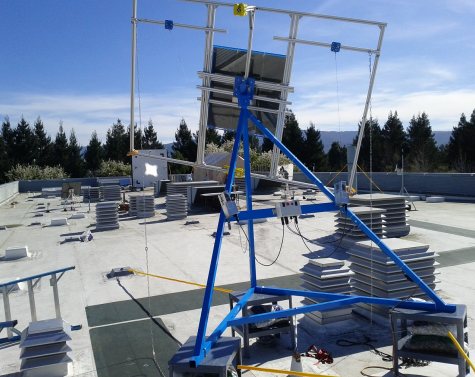
\includegraphics{HeliostatoGoogle}

Un helióstato prototipo manteniendo la luz en el objetivo. [46]

Introducción.

RE\textless C fue una iniciativa de Google para impulsar la innovación en energía renovable, con el objetivo de hacer que la energía renovable sea lo suficientemente barata para competir cara a cara con las centrales eléctricas de carbón.

Las plantas de energía solar concentradas (CSP) usan espejos o lentes para enfocar una gran cantidad de luz solar sobre un objetivo que absorbe calor, llamado receptor. El intercambiador de calor del receptor crea vapor a alta presión, que luego impulsa una turbina para alimentar un generador eléctrico. La refrigeración por agua en spray se utiliza normalmente para condensar el vapor.

La CSP modular de "torre de energía" utiliza un motor de turbina de gas más pequeño (Brayton) para realizar la conversión de energía. Los motores Brayton no necesitan refrigeración por rociado con agua y, de ese modo, se adaptan mejor a los ambientes secos del desierto.

El otro componente principal de una planta de energía CSP es un campo de espejos controlados, llamados helióstatos. Este campo tiene miles de metros cuadrados de helióstatos que concentran la energía solar en el receptor de la central eléctrica.

Nuestro diseño del helióstato.

El módulo reflector.

Cada helióstato tenía un espejo de enfoque de 2m x 3m articulado en la parte superior de su marco. El módulo reflector del espejo estaba hecho de vidrio.

El marco del helióstato y la base.

Muchos marcos y bases de helióstatos existentes son estructuras sólidas montadas sobre una base de hormigón vertido en un sitio plano. Utilizan accionamientos de precisión y grandes actuadores para realizar apuntamientos rígidos. Fue sujetado por un anclaje de tierra. Montados en el bastidor había dos accionadores de cable que usaban pequeños motores baratos.

El diseño del campo.

Cada uno de nuestros sistemas modulares de conversión de potencia del motor Brayton fue diseñado para producir una salida eléctrica planificada de 890kW por torre.

Establecimos un tamaño de campo de 862 helióstatos alrededor de una torre de 44 m, cada helióstato es de aproximadamente 6m2. Los helióstatos tienen disposición hexagonal.

Requisitos de focalización del sistema de control.

Para convertir la energía de manera eficiente, el motor Brayton requiere un receptor de cavidad de temperatura más alta que el receptor típico de una planta de vapor.

Un receptor de mayor temperatura requiere una abertura más pequeña para reducir la pérdida de calor radiante.

Sistema de detección y control.

El sistema de control es capaz de controlar simultáneamente los puntos de luz desde múltiples helióstatos a un alto grado de precisión a un lugar deseado en un objetivo.

Se utilizó un acelerómetro de 3 ejes montado en helióstato de bajo costo combinado con un sistema central de fotometría multiscópica para resolver las posiciones de puntos de luz individuales en el objetivo.

Mitigación del viento.

Las áreas de tierra grandes y planas donde es más probable que se construyan los helióstatos son también las áreas más propensas al viento.

Los helióstatos a lo largo del borde exterior de un campo protegen a los helióstatos en el medio de gran parte del impacto del viento. Las cercas de viento simples también reducen el impacto del viento en los helióstatos. [43]



\subsection{Torres CESA y CRS de la Plataforma Solar de Almería.}

La instalación CESA-1 de 7MWt


Instalación CESA. [47]

El proyecto CESA-I fue promovido por el Ministerio de Industria y Energía de España e inaugurado en mayo de 1983 para demostrar la viabilidad de las plantas solares de receptor central y para permitir el desarrollo de la tecnología necesaria. En la actualidad CESA-I ya no produce electricidad, sino que se opera, con un alto grado de flexibilidad, como una instalación de ensayo de componentes y subsistemas como helióstatos y receptores solares.
La instalación capta la radiación solar directa por medio de un campo de 300 helióstatos.
La torre es de hormigón y tiene una altura de 80 m, siendo capaz de soportar una carga de 100 toneladas. A lo largo de la torre hay tres niveles de ensayo:
Una cavidad adaptada para su uso como horno solar y ensayo de materiales.
Una cavidad con un banco calorimétrico de ensayo de receptores volumétricos presurizados.
Una instalación de ensayo de receptores volumétricos atmosféricos.
La torre se completa con una grúa en la parte superior con 5 toneladas de capacidad y un elevador montacargas con capacidad para 1.000 kg. [49]



La instalación SSPS-CRS de 2,5 MWt


Instalación CRS. [48]

La planta SSPS-CRS fue inaugurada como parte del proyecto SSPS (Small Solar Power Systems) de la Agencia Internacional de la Energía en Septiembre de 1981.
Es una instalación de ensayos dedicada al ensayo de pequeños receptores solares. El campo de helióstatos está formado por 91 unidades, aunque también existe un segundo campo con 20 helióstatos.
El campo de helióstatos CRS ha sido recientemente mejorado con la conversión de todos sus helióstatos en unidades autónomas. En la actualidad, la instalación CRS dispone del primer campo de helióstatos autónomos, que no precisa del uso de zanjas ni cableados.
La torre, de 43 m de altura, es metálica y dispone de tres plataformas de ensayo.
La infraestructura de la torre se completa con una grúa con capacidad para 4.000 kg y un elevador de cremallera con capacidad para 1.000 kg.
Para la caracterización del mapa de flujo de la radiación solar concentrada en ambas torres, se utilizan dos sistemas de medida de flujo: directo e indirecto. El sistema de medida directo consiste en una serie de calorímetros con tiempos de respuesta de microsegundos; están dispuestos en una barra móvil y montada frente a la apertura del receptor. El sistema de medida indirecto consta de una cámara CCD que utiliza un sensor de flujo para la calibración convirtiendo la escala de gris de las imágenes tomadas por la cámara en valores de flujo. [50]



\section{El lenguaje de programación Python.}

Historia
Python fue creado a finales de los ochenta por Guido van Rossum en el Centro para las Matemáticas y la Informática (CWI, Centrum Wiskunde e Informatica), en los Países Bajos.
El nombre del lenguaje proviene de la afición de su creador por los humoristas británicos Monty Python.
Van Rossum es el principal autor de Python.
En 1991, van Rossum publicó el código de la versión 0.9.0 en alt.sources. En esta etapa del desarrollo ya estaban presentes clases con herencia, manejo de excepciones, funciones y los tipos modulares, como: str, list, dict, entre otros. Además en este lanzamiento inicial aparecía un sistema de módulos adoptado de Modula-3. El modelo de excepciones en Python es parecido al de Modula-3, con la adición de una cláusula else. En el año 1994 se formó comp.lang.python, el foro de discusión principal de Python, marcando un hito en el crecimiento del grupo de usuarios de este lenguaje.
Python alcanzó la versión 1.0 en enero de 1994. Una característica de este lanzamiento fueron las herramientas de la programación funcional: lambda, reduce, filter y map.
La última versión liberada proveniente de CWI fue Python 1.2. En 1995, van Rossum continuó su trabajo en Python en la Corporation for National Research Initiatives (CNRI) en Reston, Virginia, donde lanzó varias versiones del software.
Durante su estancia en CNRI, van Rossum lanzó la iniciativa Computer Programming for Everybody (CP4E), con el fin de hacer la programación más accesible a más gente, con un nivel de 'alfabetización' básico en lenguajes de programación.
En el año 2000, el equipo principal de desarrolladores de Python se cambió a BeOpen.com para formar el equipo BeOpen PythonLabs. CNRI pidió que la versión 1.6 fuera pública, continuando su desarrollo hasta que el equipo de desarrollo abandonó CNRI; su programa de lanzamiento y el de la versión 2.0 tenían una significativa cantidad de traslapo.​ Python 2.0 fue el primer y único lanzamiento de BeOpen.com. Después que Python 2.0 fuera publicado por BeOpen.com, Guido van Rossum y los otros desarrolladores de PythonLabs se unieron en Digital Creations.
Python 2.0 tomó una característica mayor del lenguaje de programación funcional Haskell: listas por comprensión. La sintaxis de Python para esta construcción es muy similar a la de Haskell, salvo por la preferencia de los caracteres de puntuación en Haskell, y la preferencia de Python por palabras claves alfabéticas. Python 2.0 introdujo además un sistema de recolección de basura capaz de recolectar referencias cíclicas.
Posterior a este doble lanzamiento, y después que van Rossum dejara CNRI para trabajar con desarrolladores de software comercial, quedó claro que la opción de usar Python con software disponible bajo GNU GPL era muy deseable. La licencia usada entonces, la Python License, incluía una cláusula estipulando que la licencia estaba gobernada por el estado de Virginia, por lo que, bajo la óptica de los abogados de Free Software Foundation (FSF), se hacía incompatible con GPL. CNRI y FSF se relacionaron para cambiar la licencia de software libre de Python para hacerla compatible con GPL. En el año 2001, van Rossum fue premiado con FSF Award for the Advancement of Free Software.
Python 1.6.1 es esencialmente el mismo que Python 1.6, con unos pocos arreglos de bugs, y con una nueva licencia compatible con GPL.
Python 2.1 fue un trabajo derivado de Python 1.6.1, así como también de Python 2.0. Su licencia fue renombrada a: Python Software Foundation License. Todo el código, documentación y especificaciones añadidas, desde la fecha del lanzamiento de la versión alfa de Python 2.1, tiene como dueño a Python Software Foundation (PSF).
Una innovación mayor en Python 2.2 fue la unificación de los tipos en Python (tipos escritos en C), y clases (tipos escritos en Python) dentro de una jerarquía. Esa unificación logró un modelo de objetos de Python puro y consistente. También fueron agregados los generadores que fueron inspirados por el lenguaje Icon.
Las adiciones a la biblioteca estándar de Python y las decisiones sintácticas fueron influenciadas fuertemente por Java en algunos casos: el package logging, introducido en la versión 2.3, está basado en log4j; el parser SAX, introducido en 2.0; el package threading, cuya clase Thread expone un subconjunto de la interfaz de la clase homónima en Java.
Modo interactivo
El intérprete de Python estándar incluye un modo interactivo en el cual se escriben las instrucciones en una especie de intérprete de comandos: las expresiones pueden ser introducidas una a una, pudiendo verse el resultado de su evaluación inmediatamente, lo que da la posibilidad de probar porciones de código en el modo interactivo antes de integrarlo como parte de un programa. Esto resulta útil tanto para las personas que se están familiarizando con el lenguaje como para los programadores más avanzados.
Existen otros programas, tales como IDLE, bpython o IPython, que añaden funcionalidades extra al modo interactivo, como el autocompletado de código y el coloreado de la sintaxis del lenguaje.
Ejemplo del modo interactivo:
\textgreater\textgreater\textgreater 1 + 1
2
\textgreater\textgreater\textgreater a = range(10)
\textgreater\textgreater\textgreater print(list(a))
[0, 1, 2, 3, 4, 5, 6, 7, 8, 9]
[41]



\section{Usos de Python.}

Es una gran multiplataforma
Python es un lenguaje de programación interpretado, por lo que funciona en cualquier tipo de sistema que integre su interpretador.  A parte de esta ventaja, Python nos ofrece dialectos como el ya conocido Jython, que se utiliza para escribir en Java.
 
Frameworks de gran utilidad
Python no sólo es multiplataforma y multiparadigma, sino que también nos servirá para desarrollar cualquier tipo de vía, como por ejemplo web o móvil. Para que esto se lleve a cabo, este lenguaje de programación cuenta con frameworks de gran calibre, los cuales auxilian desde el desarrollo web, hasta el desarrollo de juegos o algoritmos científicos de cálculos avanzados.
 
Es libre y nos ofrece código abierto
Si hablamos de la licencia que posee, ésta es Python Software Foundation License, licencia muy parecida a la de GPL, pero encontrando la excepción de que se pueden distribuir los binarios del lenguaje sin tener que anexar las fuentes.
 
Empresas de alto prestigio utilizan Python para programar todo tipo de aplicaciones y servicios
Python se encuentra en multitud de aplicaciones y servicios que usamos habitualmente. Ostenta una gran lista de usuarios de gran calibre como Google, YouTube o Facebook, los cuales utilizan este lenguaje de programación. Poco a poco Python va ganando territorio y, entre los entendidos, se ha convertido en uno de los lenguajes más solicitados y, sobretodo, más esenciales del momento. 
Gran calidad en su sintaxis
La sintaxis que nos ofrece este lenguaje de programación es una de sus características más notorias. En Python, un bloque de código interno como puede ser un ‘if’, se crea a través de indentaciones, lo que fuerza al desarrollador a indentar su código fuente garantizando una legibilidad notoria.
Otras de sus funciones son las de reducir el uso de caracteres como ‘=’, ‘{’, ‘}’, entre otros, y de ser capaz de escribir un ‘for’ que testee una determinada secuencia.
 
Python: programación orientada a objetos
Si hablamos de programación orientada a objetos, podemos decir que nos encontramos ante un paradigma que propone modelar todo en función a clases y a objetos, el cual nos ofrece un uso de conceptos de cohesión, polimorfismo, herencia, abstracción y mucho más.
Este paradigma de programación se utiliza para tratar el rápido aumento en el tamaño y la complejidad de los sistemas de software, y facilitar la modificación de esos grandes y complicados sistemas a lo largo del tiempo.
 
Nos ofrece un tipado dinámico fuerte
Por último, cabe destacar la fácil atribución de una variable que nos ofrece a cualquier tipo de valor, y lo mejor de todo, en cualquier lugar de su código fuente.
[42]


\section{Versiones de Python.}

Guido van Rossum ideó el lenguaje Python a finales de los 80 y comenzó a implementarlo en diciembre de 1989. En febrero de 1991 publicó la primera versión pública, la versión 0.9.0. La versión 1.0 se publicó en enero de 1994, la versión 2.0 se publicó en octubre de 2000 y la versión 3.0 se publicó en diciembre de 2008. El desarrollo de Python lo lleva a cabo un colectivo de programadores que trabaja bajo el paraguas de la fundación Python Software Foundation, pero Guido van Rossum sigue dirigiendo el desarrollo de Python.
Las versiones de Python se identifican por tres números X.Y.Z, en la que:
X corresponde a las grandes versiones de Python (1, 2 y 3), incompatibles entre sí:
Los principales cambios introducidos en Python 2 fueron las cadenas Unicode, las comprensiones de listas, las asignaciones aumentadas, los nuevos métodos de cadenas y el recolector de basura para referencias cíclicas.
Los principales cambios introducidos en Python 3 fueron la separación entre cadenas Unicode y datos binarios, la función print(), cambios en la sintaxis, tipos de datos, comparadores, etc.
Por el momento, no hay planes de crear una nueva versión Python 4, incompatible con las anteriores.
Y corresponde a versiones importantes en las que se introducen novedades en el lenguaje pero manteniendo la compatibilidad (salvo excepciones).
Desde hace unos años, las versiones X.Y se publican aproximadamente cada año y medio y se mantienen durante cinco años, excepto la versión 2.7, que se mantendrá por lo menos durante diez años, hasta 2020.
Z corresponde a versiones menores que se publican durante el período de mantenimiento, en las que sólo se corrigen errores y fallos de seguridad.
Normalmente, se publica una última versión X.Y.Z justo antes de que una versión X.Y deje de mantenerse. Algunas empresas comerciales ofrecen el mantenimiento de versiones antiguas una vez acabado el mantenimiento oficial.
La imagen siguiente muestra la fecha de publicación de las versiones principales de Python, en cada una de las tres grandes versiones, Python 1, Python 2 y Python 3. Las versiones indicadas con punto rojo se consideran obsoletas, las versiones indicadas con punto negro siguen publicando actualizaciones, las versiones indicadas con punto blanco corresponden a versiones futuras con fechas ya previstas.

La imagen siguiente muestra la fecha de publicación de las últimas versiones menores de Python. Las versiones indicadas en rojo se consideran obsoletas, las versiones indicadas con punto blanco corresponden a versiones futuras con fechas ya previstas.

Es posible tener instalados en el ordenador varias versiones de Python pero, salvo que sea necesario para la ejecución de programas o paquetes incompatibles, se recomienda instalar siempre la última versión disponible.
Referencias
Principales novedades en Python (documentación oficial):
Python 2.X: 2.0 - 2.1 - 2.2 - 2.3 - 2.4 - 2.5 - 2.6 - 2.7
Python 3.X: 3.0 - 3.1 - 3.2 - 3.3 - 3.4 - 3.5 - 3.6 - 3.7
Planificación de la publicación de cada versión (release schedules):
Python 2.X: 2.6 - 2.7 - 2.8
Python 3.X: 3.0 - 3.1 - 3.2 - 3.3 - 3.4 - 3.5 - 3.6 - 3.7 - 3.8
Sobre los cambios en Python 3 (Nick Coghlan)
Cool New Features in Python 3.7, de Geir Arne Hjelle (27/06/18)
Transición de Python 2 a Python 3
La transición de Python 2 a Python 3 ha resultado mucho más costosa de lo esperado, debido a que Python 3 introdujo muchos cambios en el lenguaje y obligaba a reescribir prácticamente todos los programas (aunque se han creado herramientas para ayudar en ese proceso).
La intención inicial era haber terminado Python 2 con la versión 2.6, pero en 2010 se tuvo que publicar la versión 2.7, incorporando parte de las novedades de Python 3. Además, el período de mantenimiento de Python 2.7 se tuvo que duplicar de los cinco años habituales a diez, hasta 2020.

Un primer obstáculo en el proceso de transición de Python 2 a Python 3 ha sido la propia disponibilidad de Python 3 en las distribuciones GNU/Linux. Muchas herramientas internas de las distribuciones están escritas en Python y su conversión de Python 2 a Python 3 no era fácil, por lo que las distribuciones no podían pasar simplemente de incluir una versión a otra.
Hasta 2015, Python 2 siguió siendo la versión predeterminada de Python en la mayoría de distribuciones GNU/Linux (aunque se podía instalar Python 3 sin problemas en ellas). Felizmente, esta situación está en vías de solución:
Fedora hizo la transición a Python 3.4 en Fedora 23 (publicada en noviembre de 2015) [wiki de Fedora]. Eso quiere decir que RedHat Linux 8 (sin fecha de publicación prevista) usará Python 3. Posteriormente, Fedora 24 (publicada en junio de 2016) incluyó Python 3.5 y Fedora 26 (publicada en julio de 2017) incluyó Python 3.6.
Ubuntu hizo la transición a Python 3.5 en Ubuntu 16.04 (publicada en abril de 2016) [wiki de Ubuntu] e incluye Python 3.6 en Ubuntu 18.04 (publicada en abril de 2018) [wiki de Ubuntu].
En abril de 2015 Debian empezó a discutir los planes de transición a Python 3. Debian 9 (publicado en junio de 2017) incluye Python 2.7.13 y Python 3.5.3 y Debian 10 (que se espera publicar en 2019) debería pasar completamente a Python 3 [artículo de Linux Week News del 29/04/15].
OpenStack, una importante plataforma de virtualización, incluyó soporte para Python 3 (concretamente, Python 3.5) en la versión Pike, publicada en agosto de 2017
Aunque las nuevas versiones de las distribuciones ya incluyan Python 3, las distribuciones que incluyen Python 2 seguirán instaladas en servidores durante bastantes años. Ese es el motivo por el que se vayan a seguir publicando actualizaciones de seguridad de Python 2.7 hasta 2020, como mínimo.

Un segundo obstáculo en el proceso de transición de Python 2 a Python 3 (y que ha afectado además a todos los sistemas operativos) ha sido la disponibilidad de las bibliotecas.
Python cuenta con un gran número de bibliotecas, cuyo repositorio oficial es PyPI (Python Package Index), que facilitan la programación de aplicaciones complejas. Cuando se publicó Python 3, la inmensa mayoría de bibliotecas sólo estaban disponibles para Python 2 y, lógicamente, si un programa necesitaba alguna biblioteca que sólo estaba disponible para Python 2, el programa no se podía pasar tampoco a Python 3.
Poco a poco, la mayoría de bibliotecas de Python han ido publicando versiones para Python 3, por lo que este problema también está en vías de solución.
En marzo de 2016, un estudio de empleados de Microsoft señalaba que por aquel entonces algo más del 50\% de las bibliotecas estaban disponibles tanto para Python 2 como para Python 3, un 25\% estaban disponibles sólo para Python 2 y un poco menos del 25\% estaban disponibles sólo para Python 3, pero la tendencia parecía indicar que a mediados de 2016 Python 3 pasaría a ser la versión más popular.
Varias páginas web hacen un seguimiento de la compatibilidad con Python 3 de las bibliotecas más populares
Python 3 Wall of Superpowers (parece que desde abril de 2018 esta web ya no actualiza los datos) y Python 3 Readiness muestran cómo la inmensa mayoría de las bibliotecas más populares ya están disponibles en Python 3
la distribución GNU/Linux Fedora lleva el seguimiento de los paquetes de Python que forman parte de la distribución: paquetes y evolución.
Drop Python muestra las bibliotecas más populares han dejado de dar soporte a las versiones obsoletas de Python (Python 2.6, Python 3.2 y Python 3.3). [39]


\section{La biblioteca OpenCV.}

OpenCV (Open Source Computer Vision Library) se lanza bajo licencia BSD y, por lo tanto, es gratuito tanto para uso académico como comercial. Tiene interfaces C ++, Python y Java y es compatible con Windows, Linux, Mac OS, iOS y Android. OpenCV fue diseñado para la eficiencia computacional y con un fuerte enfoque en aplicaciones en tiempo real. Escrito en C / C ++ optimizado, la biblioteca puede aprovechar el procesamiento de múltiples núcleos. Habilitado con OpenCL, puede aprovechar la aceleración de hardware de la plataforma informática heterogénea subyacente.

Adoptado en todo el mundo, OpenCV tiene más de 47 mil personas de usuarios y una cantidad estimada de descargas que supera los 14 millones. El uso va desde el arte interactivo hasta la inspección de minas, la costura de mapas en la web o la robótica avanzada. [33]


OpenCV, es una biblioteca informática de código abierto desarrollado originalmente por la visión de Intel . Es gratuito para uso comercial y la investigación bajo un licencia BSD. La biblioteca es multiplataforma y funciona en Mac OSX, Windows y Linux. Se centra principalmente hacia procesamiento imagen tiempo real como tal si encuentra Intel Integrated Performance Primitives sobre el sistema, utilizará estas rutinas optimizado comerciales a acelerarse.
Diseño del proyecto
Lanzado oficialmente en 1999, el proyecto


OpenCV
fue inicialmente OpenCV iniciativa de investigación del Intel para avanzar en la CPU aplicaciones de uso intensivo, que forma parte de una serie de proyectos, entre ellos en tiempo real el trazado de rayos y las paredes de visualización 3D.Los principales contribuyentes al proyecto incluye equipo de Intel la biblioteca de rendimiento. En los primeros días de OpenCV, los objetivos del proyecto se describe como:
Avanzar en la investigación, proporcionando la visión no sólo libre, sino también el código optimizado para las infraestructuras básicas de la visión.
Difundir el conocimiento de la visión de aportar una infraestructura común que los desarrolladores pueden construir, para que el código sería más fácil lectura e intransferible.
Promover la visión basada en aplicaciones comerciales, haciendo portátiles, rendimiento optimizado de código disponible de forma gratuita con una licencia que no requiere ser abierto o gratuitas.
Historia
Desde que apareció su primera versión alfa en


Proyecto
el mes de enero de 1999, se ha utilizado en infinidad de aplicaciones. Desde sistemas de seguridad con detección de movimiento, hasta aplicativos de control de procesos donde se requiere reconocimiento de objetos. Esto se debe a que su publicación se da bajo licencia BSD, que permite que sea usada libremente para propósitos comerciales y de investigación con las condiciones en ella expresadas.
OpenCV es multiplataforma, existiendo versiones para GNU/Linux, Mac OSX y Windows. Contiene más de 500 funciones que abarcan una gran gama de áreas en el proceso de visión, como reconocimiento de objetos (reconocimientos facial), calibración de cámaras, visión estéreo y visión robótica.
El proyecto pretende proporcionar un entorno de desarrollo fácil de utilizar y altamente eficiente. Esto se ha logrado, realizando su programación en código C y C++ optimizados, aprovechando además las capacidades que proveen los procesadores multi núcleo. OpenCV puede además utilizar el sistema de primitivas de rendimiento integradas de Intel, un conjunto de rutinas de bajo nivel específicas para procesadores Intel (IPP).
Funciones
Captura en tiempo real.
Importación de archivos de vídeo.
El tratamiento básico de imágenes (brillo, contraste, umbral).
Detección de objetos (cara, cuerpo).
Blob detección.
Aplicaciones
OpenCV ha sido usado en el sistema de visión del vehículo no tripulado Stanley de la Universidad de Stanford, el ganador en el año 2005 del Gran desafío DARPA
OpenCV se usa en sistemas de vigilancia de vídeo
OpenCV es la clave en el programa Swistrack, una herramienta de seguimiento distribuida
Lenguaje de programación
La biblioteca fue originalmente escrita en C y esta interfaz C hace OpenCV portátil para algunas plataformas específicas,tales como procesadores de señal digital.
OpenCV incluye tanto la interfaz de C tradicionales, así como una nueva interfaz C++, que busca reducir el número de líneas de código necesarias al código de la funcionalidad de la visión, así como reducir los errores comunes de programación, tales como la memoria fugas que pueden surgir al utilizar OpenCV en la mayoría de los nuevos desarrollos y algoritmos OpenCV C.
Se desarrollan en el interfaz C++, es mucho más difícil para las envolturas en otras lenguas de código C++ en lugar de código en C. [36] [37] [38]


\section{Trabajo realizado en el proyecto.}

\section{Variables de entorno.}

Antes de trabajar el código, hay que agregar unas variables de entorno en el sistema.

Para ello, se hace clic en Inicio, situado en la esquina inferior izquierda de la pantalla, y teclear ‘Variables de entorno’ para buscar esta configuración. Hacer clic en ‘Editar las variables de entorno del sistema’, el resultado que aparecerá. Y en la ventana que se abrirá, hacer clic en ‘Variables de entorno’.

Por si acaso, en mi caso particular, he agregado las variables de entorno tanto para mi propio usuario como para el sistema completo. Las variables de entorno que deberán agregarse son:

Variable: Python35-32. Valor: C: \textbackslash Users \textbackslash Pc \textbackslash AppData \textbackslash Local \textbackslash Programs \textbackslash Python \textbackslash Python35-32.
Variable: Python36. Valor: C: \textbackslash Users \textbackslash Pc \textbackslash AppData \textbackslash Local \textbackslash Programs \textbackslash Python \textbackslash Python36.

(Siendo ‘Pc’ el nombre de mi usuario; aquí se debe introducir el nombre de usuario correspondiente.)

Para agregar una variable de entorno, hacer clic en ‘Nueva...’. Hay dos botones ‘Nueva...’. El que se ubica arriba se agrega en el usuario específico del sistema, y el que se ubica abajo se agrega para todo el sistema en general. En ‘Nombre de la variable’ y ‘Valor de la variable’, introducir los datos mencionados anteriormente, y hacer clic en ‘Aceptar’.




\section{Instalación del software Python.}

Para este trabajo de fin de grado, se necesitaba desarrollar un software usando un programa de ordenador: Python. La última versión disponible a la hora de realizar dicho trabajo era la 3.6.4. Se ha utilizado además la versión de 64 bits, debido a que mi PC donde desarrollé el programa monta esta arquitectura de CPU.

A continuación, se explicará cómo descargar Python 3.6.4.

Abrir un explorador de internet como Google Chrome, y buscar en Google ‘Instalar Python 3.6.4 64 bits’. Pinchar en el resultado ‘Python Release Python 3.6.4 | Python.org’.



Una vez se haya accedido a esa página oficial de Python, realizar scroll hacia abajo para acceder a los archivos disponibles de esa versión de Python a descargar en el PC.



Pinchar en ‘Windows x86-64 executable installer’ para descargar en el PC el instalador de Python, el cual se encargará de instalar este programa.



La descarga se completará en cinco segundos. Pinchar en el archivo ‘EXE’ mostrado en la esquina inferior izquierda para abrir el instalador de Python.



Aparecerá esta ventana de instalación. A no ser que se desee agregar manualmente las variables de entorno de Python (con el fin de poder ejecutar Python desde la consola de comandos de Windows), hacer clic en ‘Add Python 3.6 to PATH’. El propio instalador llevará a cabo este procedimiento. A continuación, hacer clic en ‘Install Now’.



Se instalará Python en el sistema. Hay que esperar unos minutos para que este procedimiento se complete (cuando la barra verde se llene por completo).



Cuando finalice correctamente la instalación, se mostrará en la ventana del instalador ‘Setup was successful’. Hacer clic en ‘Close’ para cerrar el instalador.



El icono de Python debería aparecer en el escritorio. Hacer doble clic para abrir el programa.



Si no aparece el icono de Python en el escritorio, hacer clic en el logotipo (o bandera) de Windows mostrado en la esquina inferior izquierda de la pantalla, y teclear ‘idle’. Debería ya aparecer en el buscador de programas ‘IDLE (Python 3.6 64-bit)’. Hacer clic ahí para abrirlo.



En el caso de querer agregar el icono del programa al escritorio (si no lo estaba), desde esa misma pantalla del buscador de programas, situar el cursor sobre el programa, hacer clic con el botón derecho del ratón, y seleccionar ‘Abrir ubicación de archivo’. Se mostrará la ubicación exacta del archivo en el sistema, abriéndose la ventana del explorador de archivos de Windows.



Desde esa ventana, y haciendo clic con el botón derecho del ratón sobre el programa (acceso directo) ‘IDLE (Python 3.6 64-bit)’, seleccionar desde el menú contextual ‘Crear acceso directo’. Se creará un nuevo acceso directo a ese programa, en esta misma ventana, con nombre ‘IDLE (Python 3.6 64-bit) (2)’.



Reducir el tamaño de la ventana, de forma parecida a la mostrada en esta captura de pantalla. Tras esto, simplemente habría que arrastrar y soltar este acceso directo ‘IDLE (Python 3.6 64-bit) (2)’ desde esa ventana al escritorio. Así, ya se tiene el programa en el escritorio.


\section{Cómo usar el software.}

Para usar y ejecutar el software en el PC descrito en este informe, especialmente por primera vez, se siguen las siguientes instrucciones:

\# Heliostatos

--- Cómo abrir y ejecutar el proyecto de caracterización de helióstatos ---

Nota: el código de este proyecto se realizó mediante el programa Python e IDLE 3.6.4.

1. Acceder a la página Web donde se ubica el proyecto: https://github.com/VictorRodri/Heliostatos
2. En ella, hacer clic en el botón verde 'Clone or download' \textgreater 'Download ZIP'.
3. El proyecto se descargará en el disco duro del equipo, generalmente en 'Documentos' \textgreater 'Descargas'. De lo contrario, especificar en qué ruta exacta del equipo se realizará la descarga.
4. Descomprimir el proyecto descargado previamente, usando un software como WinRAR: https://www.winrar.es/descargas
5. Instalar la última versión de Python desde su página Web oficial: https://www.python.org/downloads/
6. Abrir la terminal de comandos de Windows. Para ello, hacer clic en 'Inicio' \textgreater 'Ejecutar'. En la ventana que aparecerá, escribir en el cuadro de texto 'cmd' y pulsar Enter.
7. La terminal mostrará la ruta o directorio del sistema donde se ubica usted actualmente, como 'C: \textbackslash Users \textbackslash Pc\textgreater'. Ir navegando hasta encontrar el directorio que contiene el proyecto descomprimido previamente. Para acceder a una carpeta, escribir 'cd NombreCarpeta' y pulsar Enter. Para salir del directorio actual, escribir 'cd ..'.
8. Una vez se haya navegado al directorio que contiene el proyecto, ejecutarlo con el comando 'estimacion\_potencia.py Videos/varios\_heliostatos.mp4 50 50', siendo respectivamente el nombre del proyecto '.py' con el software ejecutable, el directorio que contiene el vídeo de helióstatos a ser procesado, y el ancho y alto mínimos del helióstato para su detección y análisis.
9. Durante aproximadamente un minuto, se ejecutará el software que consistirá en medir la radiación de energía que proyecta cada helióstato. Concretamente, la energía se calcula como la sumatoria de los cuadrados de cada componente BGR del helióstato. Aparecerán estos resultados en tiempo de ejecución en la consola, para cada fotograma del vídeo de helióstatos.
10. Si desea cancelar la ejecución del software, pulsar 'Ctrl+C'.


\section{Diagrama de flujo.}

El funcionamiento del código de helióstatos mediante la representación de un diagrama de flujo es el siguiente:






 
\section{Funcionamiento del software y código.}

El software consiste en la lectura y procesamiento de un vídeo guardado en el disco duro del ordenador personal y en formato MP4. El vídeo es de un conjunto de helióstatos que van entrando uno por uno en un panel solar y fusionándose todos entre sí. Y tras esto, los helióstatos van saliendo uno por uno de ese panel solar, hasta que no quede ninguno.

El código desarrollado es el siguiente:

\# Bibliotecas requeridas para este software.
import cv2
import argparse
import time
import numpy as np

Para que funcione todo el código expuesto y elaborado a continuación, hay que importar en este caso las librerías ‘cv2’, ‘argparse’ y ‘numpy’ (esta última se ha asignado un nombre propio: ‘np’).

‘cv2’ permite el uso de distintas funcionalidades de Python. En este proyecto, se ha usado para la captura y lectura de un vídeo guardado en el sistema, convertirlo de color a escala de grises, aplicarle un umbral (diferenciar solo dos niveles de grises: u oscuros o claros), mostrar el vídeo original y umbralizado en pantalla y en reproducción (conforme el programa lo va analizando fotograma a fotograma), realizar pausas (breves o prolongadas) de la ejecución del código, detectar y localizar contornos (helióstatos) en el vídeo, obtener las coordenadas del contorno (ubicación del contorno en el fotograma actual del vídeo), calcular el valor del área de(l) (los) contorno(s) seleccionado(s), dibujar un rectángulo verde o de otro color alrededor del contorno en el vídeo.
‘argparse’ es usado para proporcionar distintos parámetros desde la consola de Windows al ejecutar este código. En este caso, los parámetros usados son la ruta del vídeo a cargar del sistema, y el área, ancho y alto mínimos del helióstato para ser detectado y analizado por el programa.
‘time’ permite medir tiempos de ejecución de todo el código o de fragmentos de código, en segundos. Se utilizará para medir la tasa de ‘frames’ (fotogramas) por segundo de la lectura y procesado del vídeo de helióstatos, y así comprobar la eficiencia de la ejecución del programa.
‘numpy’ permite el manejo de arrays o vectores con el fin de recorrer y analizar una serie de datos en secuencia, como una matriz de dos dimensiones y con muchos valores numéricos guardados. Además, usar ‘numpy’ para dicho fin es mucho más eficiente que otros métodos de análisis de datos en secuencia que no sean en arrays o vectores, como los típicos bucles ‘for’.


start\_time = time.time() \# Obtener el tiempo de ejecución inicial de este programa.
frame\_counter = 0 \# Contador de fotogramas totales del vídeo. Se irá incrementando progresivamente en líneas de código posteriores.

Obtener en segundos el tiempo de ejecución inicial del programa. Inicial porque esta línea de código se ubica en el comienzo del software. Declarar e inicializar a cero un contador de fotogramas del vídeo. Ambos datos serán usados para calcular los FPS (fotogramas por segundo) del vídeo de helióstatos, al final de este código.


\# Argumentos o parámetros necesarios para ejecutar este programa a través de la consola de Windows.
parser = argparse.ArgumentParser(description='Parametros del programa.') \# Dar un nombre al conjunto de parámetros y asignarlo a la variable 'parser'.
parser.add\_argument('directorioVideoHeliostatosCargar', type=str) \# Crear el argumento 1: ruta o directorio del vídeo a cargar en el PC.
parser.add\_argument('anchoMinimoHeliostato', type=int) \# Crear el argumento 3: ancho mínimo del helióstato para su análisis.
parser.add\_argument('altoMinimoHeliostato', type=int) \# Crear el argumento 4: alto mínimo del helióstato para su análisis.
args = parser.parse\_args() \# Devuelve información de los parámetros definidos previamente.

Permite que a la hora de ejecutar el programa desde la terminal de comandos de Windows, solicite al usuario la ruta del vídeo a cargar del sistema, y el ancho y alto mínimos del helióstato para ser detectado y analizado por el programa. Por ejemplo: ‘C: \textbackslash Users \textbackslash Pc \textbackslash Desktop \textbackslash TFG>miCodigo.py Videos/varios\_heliostatos.mp4 50 50’.

‘parser = argparse.ArgumentParser(description='Parametros del programa.')’. Esta línea de código permite asignar un conjunto de parámetros o argumentos y de darles un nombre. Es guardado en la variable ‘parser’.
Partiendo de la anterior variable ‘parser’, se van designando los distintos argumentos, junto a sus nombres y tipos, como cadena o entero (según si la entrada del parámetro hay que escribir letras y/o caracteres, o simplemente números).
‘args = parser.parse\_args()’. Permite que, desde la variable ‘args’, cargar el argumento concreto, almacenado previamente cuando el programa solicitó al usuario los argumentos. Por ejemplo, si se desea comprobar cuál fue el ancho del helióstato que el usuario solicitó por parámetro en la consola, se cargará y obtendrá el segundo argumento con la línea de código siguiente: ‘args.anchoMinimoHeliostato’. Así, el programa realizará las medidas y operaciones oportunas de acuerdo al valor de este parámetro deseado por el usuario.


\# Mostrar en la consola este aviso de cuando se va a ejecutar el programa.
print("")
print("Iniciando programa...")
print("")

Al iniciar la ejecución del programa, mostrará por consola que se ha iniciado su ejecución, con el aviso ‘Iniciando programa…’. Este aviso solo aparecerá una vez durante toda su ejecución.


\# Leer secuencia de imágenes del vídeo a partir del directorio especificado por parámetro.
camara = cv2.VideoCapture(args.directorioVideoHeliostatosCargar)

Partiendo del directorio especificado por el usuario, el programa leerá y cargará el archivo concreto, que deberá ser el vídeo de helióstatos. De lo contrario, la ejecución del programa no se realizará correctamente.


\# Iteración 'while True' para cada fotograma del vídeo, hasta completar todos los fotogramas y llegar al final del vídeo (cambiaría automáticamente de True a False y el bucle 'while' finaliza).
while True:

A partir de aquí y prácticamente hasta el final del código, todas las demás instrucciones se aplicarán para cada fotograma del vídeo de helióstatos.

    
    \# Obtener frame. Para ello, se toma un fotograma del vídeo, se guarda en 'frame', y si se ha hecho esta acción correctamente, 'grabbed' valdrá true (verdadero), y viceversa.
    (grabbed, frame) = camara.read()

    \# Si se ha llegado al final del vídeo, romper la ejecución de este bucle 'while' y finalizar el programa.
    if not grabbed:
        break

Estas líneas de código se encargarán de indicar al programa si quedan más fotogramas por leer o no del vídeo de helióstatos, y así saber hasta cuándo dicho programa se mantendría en ejecución. Primero, ‘camara.read()’ obtiene el fotograma actual del vídeo, y lo guarda en la variable ‘frame’. Si se ha hecho esta acción correctamente (debido a que quedan más fotogramas por leer del vídeo y no se ha llegado al final del mismo), ‘grabbed’ (justo al lado izquierdo de ‘frame’) valdrá ‘true’, y viceversa. Si se ha llegado al final del vídeo, ‘grabbed’ valdrá ‘false’ (porque ya no quedan más fotogramas por leer), y romperá la ejecución del presente bucle ‘while’ para que deje de leer más fotogramas del vídeo y finalice la ejecución de este programa. Esta ruptura es producida porque se cumple la condición de ‘if not grabbed’, así que desencadena la instrucción ‘break’.


    \# Convertir a escala de grises el fotograma actual del vídeo. Para ello, con la variable 'frame' (fotograma del vídeo) capturada anteriormente, se llama a la función 'cv2.COLOR\_BGR2GRAY'.
    img = cv2.cvtColor(frame, cv2.COLOR\_BGR2GRAY)
    
    \# Aplicar un umbral a ese fotograma del vídeo. Parámetros de este método: imagen fuente en escala de grises, valor de umbral para clasificar los valores de píxeles de esa imagen,
    \# valor máximo a ser representado si el valor del píxel supera al valor del umbral, aplicar un tipo concreto de umbralización (0 porque no se desea hacer esto).
    \# NOTA: la variable ‘ret’ que recibe como resultado en este método no es usada en este programa así que se puede ignorar, esto es debido a que no se está aplicando umbralización de Otsu.
    ret, thresh = cv2.threshold(img, 127, 255, 0)
    
    cv2.imshow("Camara2", thresh) \# Mostrar vídeo umbralizado en una ventana.

    cv2.waitKey(1) \# El programa hará una pequeña pausa (1 milisegundo) para que de tiempo a que se muestren los vídeos y fotogramas en las dos ventanas que se han creado en este código para tal fin.

    \# Buscar y detectar todos los contornos o helióstatos del fotograma actual del vídeo.
    \# Parámetros del siguiente método: imagen umbralizada, devolver todos los contornos y crear una lista completa de jerarquía de familia, marcar la mínima cantidad de puntos (no todos)
    \# que forman (delimitan) la figura (helióstato). Argumentos que devolverá dicho método: imagen fuente (sobra), modo de devolución del contorno, método de aproximación del contorno (sobra).
    im2, contours, hierarchy = cv2.findContours(thresh, cv2.RETR\_TREE, cv2.CHAIN\_APPROX\_SIMPLE)

Las siguientes líneas de código se encargarán de convertir cada fotograma del vídeo a escala de grises, aplicarle un umbral y detectar los contornos o helióstatos, así como mostrar en pantalla la visualización en vivo (al mismo tiempo que la ejecución del programa) del vídeo de helióstatos umbralizado.

Convertir a escala de grises el fotograma actual del vídeo. Basta con tomar la anterior variable ‘frame’ (fotograma actual del vídeo a color), y aplicar la línea de código ‘cv2.COLOR\_BGR2GRAY’. El fotograma convertido a escala de grises se guarda en la variable resultado ‘img’.
Aplicar un umbral al fotograma actual del vídeo en escala de grises (variable ‘img’ anterior). Un vídeo umbralizado en escala de grises permite diferenciar únicamente dos niveles de color: gris oscuro y gris claro. Así se facilitan las tareas de análisis y detección de contornos (helióstatos) en el vídeo. En este caso, el umbral definido ha sido de 127, y el máximo típico de 255. Es decir, si el píxel del vídeo es gris oscuro, en una escala de grises 0-127, será tratado y pintado como negro. En otros casos (128-255), como blanco. Así para todos los píxeles de cada fotograma del vídeo, quedando un vídeo en blanco y negro puros. Blanco es el helióstato, y negro el fondo. El fotograma umbralizado se guarda en la variable resultado ‘thresh’. Después, con el método ‘imshow’, se muestra en tiempo de ejecución y en una ventana el vídeo de helióstatos umbralizado. Es importante realizar después de las operaciones anteriores una pausa muy breve de un milisegundo para que el programa le de tiempo a mostrar los vídeos y fotogramas actualizados en las dos ventanas: vídeo normal y umbralizado. Para ello, se usa el método ‘waitKey(1)’, siendo ‘1’ el tiempo de espera deseado en milisegundos.
Buscar, detectar y delimitar todos los contornos o helióstatos del fotograma actual del vídeo umbralizado. Para ello, el método ‘findContours’ requiere de los parámetros necesarios para saber cuál es el fotograma umbralizado a tratar (variable ‘thresh’ obtenida previamente), cómo devolverá el o los resultados (en este caso devolverá todos los contornos detectados, y almacenados en lista completa de de jerarquía de familia), y cómo delimitará el contorno (en este caso usando la mínima cantidad de puntos). Los contornos detectados se guardarán en la variable resultado ‘contours’. Las otras dos variables resultado ‘im2’ e ‘hierarchy’ no son usadas para este proyecto.
        

    \# Recorrer solo los dos primeros contornos, los más grandes (siguiente bucle 'for'), para cada fotograma del vídeo (bucle 'while' ejecutándose actualmente).
    \# Al no recorrer los demás contornos, estos serán descartados porque no son muy grandes ni importantes o son falsos.
    for i in range(0,2):

Este bucle ‘for’ que va de 0 a 2 (el número 2 no se cuenta, así que solo se cuenta el 0 y el 1) se encargará de analizar únicamente los dos contornos más grandes, para cada fotograma del vídeo. De esta forma, se ignorarán los falsos contornos y menos importantes. Además, en dicho bucle se abarcan y realizan operaciones como detectar las coordenadas de cada helióstato en el vídeo, así como calcular sus áreas y sumatorias de los valores de las componentes RGB al cuadrado de todos sus píxeles.
        
        
        \# Obtener las coordenadas del contorno.
        (x, y, w, h) = cv2.boundingRect(contours[i]) \# xy: coordenadas de un punto, w: ancho, h: altura.

        \# Calcular el área del contorno numero 'i', en el fotograma actual del vídeo. 'i' es el iterador del bucle 'for' actual.
        area = cv2.contourArea(contours[i])
        
Para cada contorno, se obtendrán sus coordenadas en el vídeo, y su valor de área, aparte de mostrar el vídeo de helióstatos normal en pantalla (en tiempo de ejecución), o de actualizarlo al siguiente fotograma que se analizará.

Obtener las coordenadas del contorno usando el método ‘boundingRect’: XY, correspondientes a su esquina superior izquierda en el vídeo, y WH, correspondientes a su ancho (horizontal) y su altura (vertical). Es posible que si el helióstato todavía no ha terminado de entrar en el vídeo (desde el lado izquierdo), pues que no se muestre su esquina superior izquierda. Así que en este caso, se mostrará la esquina superior izquierda del helióstato mostrado en dicho vídeo hasta el momento. Respectivamente para el ancho y la altura.
Para el contorno número 1 y/o 2 del fotograma actual del vídeo, el programa detectará y calculará su área total, gracias al método ‘contourArea’ de la biblioteca de OpenCV.


        \# Si el contorno tiene un ancho y alto mayores a los especificados por parámetros, este será analizado y reencuadrado en un rectángulo verde en el vídeo.
        if (w > args.anchoMinimoHeliostato and h > args.altoMinimoHeliostato):

Esta condición ‘if’ solo será ejecutada si los valores que el usuario proporcionó por parámetro desde consola de ancho y alto del helióstato son menores al ancho y alto del helióstato que se va a analizar justo ahora. Si se cumplen todas, se accederá a este ‘if’ para calcular y mostrar en consola la sumatoria acumulativa de los valores de las componentes RGB al cuadrado de todos los píxeles del contorno (helióstato), además del valor de área y de reencuadrarlo en un rectángulo verde en el vídeo. Y también, se mostrarán sus coordenadas (ubicación) en el vídeo, su ancho y alto, etcétera. Todo esto se irá aplicando a cada contorno.
            

            \# Si se está analizando el contorno número uno en el fotograma actual del vídeo, hacer.
            if (i == 0):

                \# Dibujar un rectángulo verde alrededor del contorno, en el vídeo.
                \# Parámetros: fotograma actual vídeo, esquina superior izquierda, esquina inferior derecha (width: ancho, height: altura), rectángulo color verde, grosor del rectángulo 2 píxeles.
                cv2.rectangle(frame, (x, y), (x+w, y+h), (0, 255, 0), 2)

                \# Mostrar en consola que se está analizando el helióstato reencuadrado en un rectángulo verde en el vídeo.
                print("")
                print("- Analizando el helióstato verde...")
                print("")

            \# Si se está analizando el helióstato número dos en el fotograma actual del vídeo (en caso de que ya exista el otro helióstato en ese mismo fotograma del vídeo), hacer.
            else:

                \# En este caso, ahora se reencuadra el contorno en un rectángulo rojo, en vez de verde. Así, ambos contornos podrán ser diferenciados si se muestran en el mismo fotograma del vídeo.
                cv2.rectangle(frame, (x, y), (x+w, y+h), (0, 0, 255), 2)

                \# Mostrar en consola que se está analizando el helióstato reencuadrado en un rectángulo rojo en el vídeo.
                print("")
                print("- Analizando el helióstato rojo...")
                print("")

Aquí puede suceder los siguientes casos:

Si solo hay un contorno en el fotograma actual del vídeo, o hay dos pero relativamente juntos entre sí (rozándose, fusionándose o separándose), se reencuadrará en verde dicho contorno o doble contorno en el vídeo usando el método ‘rectangle’. También se mostrará en consola ‘Analizando el helióstato verde…’, queriendo decir que el procedimiento explicado a continuación de su análisis será realizado para ese contorno, o ese conjunto de contornos.
Si se muestran dos contornos separados entre sí en un mismo fotograma del vídeo, se analizarán primero uno y después el otro. En el vídeo, cada contorno se reencuadrará en colores distintos: el de la izquierda en verde y el de la derecha en rojo. Cuando se analice uno u otro contorno, aparecerá en consola ‘Analizando el helióstato verde/rojo…’, dependiendo del caso.
Si en el fotograma actual del vídeo no hay contornos, no se hará ningún procedimiento. Simplemente se pasará inmediatamente al siguiente fotograma del vídeo para seguir analizando más helióstatos que pudieran existir en ellos. No se mostrará información adicional en consola en este caso.

Además, conforme el helióstato se vaya desplazando por el vídeo, también lo hará el rectángulo verde o rojo para mantener el reencuadre.

Respecto a los parámetros introducidos en el método ‘rectangle’, aclarar que ‘x+w’ hace referencia a la esquina superior derecha del contorno, porque a ‘xy’, que es su esquina superior izquierda, se le suma su ancho ‘w’. Respectivamente para ‘y+h’ que es su esquina inferior izquierda: a ‘xy’ (esquina superior izquierda) se le suma su altura ‘h’. La combinación de las esquinas superior derecha y la inferior izquierda, ‘(x+w, y+h)’, resulta la esquina inferior derecha.


            \# Leer y analizar todos los píxeles del helióstato.
            def vectorial(frame, x, y):
                \# Del fotograma actual del vídeo, se leerá únicamente donde haya un helióstato (su ancho y alto), y así con todos los helióstatos de cada fotograma del vídeo.
                i = frame[y+2:y+h-1, x+2:x+w-1]
                
                \# Matrices BGR resultado de la lectura de ese helióstato.
                mB = i[:, :, 2]
                mG = i[:, :, 1]
                mR = i[:, :, 0]
                                
                \# Elevar al cuadrado cada dato BGR del helióstato.
                mB2 = np.power(mB, 2)
                mG2 = np.power(mG, 2)
                mR2 = np.power(mR, 2)

                \# Realizar la sumatoria acumulativa de cada BGR al cuadrado de ese helióstato.
                sumB = np.sum(mB2)
                sumG = np.sum(mG2)
                sumR = np.sum(mR2)

                \# Sumar las anteriores tres componentes entre sí, para obtener la sumatoria total de los valores de las tres componentes RGB entre sí de todos los píxeles al cuadrado del contorno entero.
                sumaRGB = sumR+sumG+sumB
                
                \# Mostrar en consola los resultados del helióstato o helióstatos localizados y analizados, para cada fotograma del vídeo.
                print("Ancho y alto WH del helióstato en píxeles:       \%4i \%4i" \%(w, h)) \# Mostrar en consola el ancho y el alto WH del helióstato en píxeles.
                print("Área del helióstato en píxeles:                  ", area) \# Mostrar en consola el área del helióstato en píxeles.
                print("Sumatorias RGB al cuadrado de todos sus píxeles: %8i %8i %8i" %(sumB, sumG, sumR))
                print("Suma total RGB al cuadrado helióstato completo:  ", sumaRGB)

            \# Llamar a la función definida 'vectorial(frame, x, y)', siendo 'frame' el fotograma actual del vídeo a tratar, y XY las coordenadas de la esquina superior izquierda del helióstato.
            vectorial(frame, x, y)
        
Estos dos bucles ‘for’ compactados en vectores son los encargados de analizar píxel a píxel el helióstato. Primero se analizarán los píxeles de columnas, y luego los de filas. En resumen, se realizan las siguientes operaciones: medir el ancho, alto y área del helióstato en píxeles, calcular para cada píxel del helióstato las componentes RGB y RGB al cuadrado (cada componente por separado), y con estas últimas, realizar una sumatoria acumulativa de cada componente RGB por separado de todos los píxeles que componen el helióstato, y después, lo mismo pero sumando o unificando las tres componentes entre sí.

Esta sección de código se ha trabajado sobretodo con NumPy (abreviado como ‘np’ en el código) y con arrays, con el fin de reducir considerablemente el tiempo de ejecución del programa. La función ‘vectorial()’ es llamada y con los parámetros ‘fotograma actual del vídeo’, y las coordenadas XY de la esquina superior izquierda del helióstato, que es desde donde se empezarán a analizar cada helióstato, hasta llegar a su esquina inferior derecha.

En la línea de código ‘i = frame[y+2:y+h-1, x+2:x+w-1]’, se obtendrá, de ese fotograma, el helióstato. Para ello, en la primera entrada de ‘frame’, que hace referencia al número de filas, se indica el número de las mismas, es decir, desde la altura máxima del helióstato ‘y’ hasta su base inferior ‘y+h’. Y en la segunda entrada de ‘frame’, correspondiente al número de columnas, se proporciona también cuántas tiene: desde el lado izquierdo ‘x’ hasta el lado derecho del helióstato ‘x+w’. Es importante no confundir la longitud/altura del helióstato (‘w’ y ‘h’, respectivamente), con las coordenadas o ubicación del helióstato en el vídeo, midiéndose desde su esquina superior izquierda (‘XY’). Para seleccionar o cargar el helióstato (variable ‘i’) del fotograma actual del vídeo (variable ‘frame’), se parte desde la esquina superior izquierda de ese helióstato con la coordenada ‘X’, y para definir el límite derecho (lado derecho) del helióstato, a esa ‘X’, que es donde está ubicado el helióstato en el vídeo, se le suma su longitud ‘w’. Y respectivamente para la altura. Indicar que, con el fin de evitar leer sobre el rectángulo verde o rojo que reencuadra al helióstato en el vídeo, se le han puesto en ‘frame’ unos números ‘+2’ y ‘-1’. Son las medidas exactas para evitar que esto suceda.

En ‘mB = i[:, :, 2], mG = i[:, :, 1], mR = i[:, :, 0]’, se obtendrán las salidas BGR (o números del 0-255) de ese helióstato cargado previamente en la variable ‘i’. Para ello, se indica, en cada matriz ‘mB’, ‘mG’ y ‘mR’ (matrices de píxeles azules, verdes y rojos del helióstato, respectivamente), que se desean obtener todas las filas y columnas de ‘i’, es decir, todos los valores BGR del helióstato. Se indican con los dos puntos ‘:’, en las dos primeras entradas de esas matrices. Y en la tercera entrada, que correspondería a la tercera dimensión, se obtienen los valores azules ‘B’ con el número 2, los verdes ‘G’ con el 1, y los rojos ‘R’ con el 0.

Con esos valores BGR (‘mB’, ‘mG’ y ‘mR’), se elevarán cada uno de ellos al cuadrado con el método ‘np.power’. Así, se dispondrán en ‘mB2’, ‘mG2’ y ‘mR2’ todos los valores BGR del helióstato elevados al cuadrado. Los valores RGB solo pueden ser representados del 0 al 255. Al elevar al cuadrado unos de estos valores, nunca se sobrepasará del 255, y pasará del 255 al cero directamente, y así sucesivamente. Esto lo realiza el programa automáticamente.

Con todos estos valores BGR del helióstato elevados al cuadrado, se realizará una sumatoria acumulativa de todos ellos, para cada componente BGR por separado. Los resultados de las sumatorias se guardarán en ‘sumB’, ‘sumG’ y ‘sumR’. Se trataría de cumplir la siguiente fórmula:

E = sumatoria R al cuadrado + sumatoria G al cuadrado + sumatoria B al cuadrado
Siendo ‘sumatoria’ la sumatoria acumulativa de todos los píxeles del helióstato.

Para cada helióstato, se obtendría entonces: Er, Eg y Eb.
           
Finalmente, en ‘sumaRGB = sumR+sumG+sumB’, esta acción consiste en sumar o unificar los resultados ‘sumB’, ‘sumG’ y ‘sumR’ obtenidos previamente (las anteriores sumatorias al cuadrado de todos los píxeles del contorno). Así, lo que se estaría haciendo para cada helióstato sería lo siguiente:

Etotal = Er + Eg + Eb

Es decir, obtener la sumatoria total de los valores de las tres componentes RGB entre sí de todos los píxeles al cuadrado del contorno entero.

Mostrar en consola el valor del área del helióstato en píxeles, su ancho y alto también en píxeles, los valores de las sumatorias acumulativas RGB al cuadrado (cada componente por separado) de todos los píxeles del helióstato, y esto mismo pero sumando esta vez las tres componentes entre sí.

Cuando se analiza otro helióstato (independientemente de si se salta o no al siguiente fotograma del vídeo), los valores de área y sumatorias pasarán automáticamente a valer cero de partida. De esta forma, no se obtendrán valores de un helióstato acumulados (erróneos) del helióstato analizado previamente.


\# Mostrar vídeo original en una ventana/actualizar fotograma.
cv2.imshow("Camara", frame)

Mostrar el vídeo de helióstatos normal en pantalla con el método ‘imshow()’, y reproducirse al mismo tiempo que el programa va analizando cada uno de sus fotogramas. Con ‘reproducirse’, quiere decir además que se actualizará o cambiará el fotograma del vídeo al actual.


\# Al alcanzar esta línea de código, ya se habrá leído y analizado el fotograma actual del vídeo. Antes de pasar al siguiente fotograma, hacer:
    frame\_counter += 1 \# Incrementar el contador de fotogramas leídos del vídeo a uno.
    end\_time = time.time() \# Obtener el tiempo de ejecución tras haber leído el fotograma actual del vídeo.
    fps = frame\_counter / float(end\_time - start\_time) \# Calcular los FPS (fotogramas por segundo del vídeo) dividiendo el contador de fotogramas actual por la diferencia entre ambos tiempos medidos.
    print("FPS:", fps) \# Mostrar en consola los FPS (fotogramas por segundo del vídeo). Se mostrará cada vez que se haya analizado el fotograma actual del vídeo.

Esta sección de código se encargará de calcular los FPS (fotogramas por segundo) del vídeo de helióstatos, cada vez que se lea y analice un fotograma completo de ese vídeo (o el equivalente a haber alcanzado estas líneas de código). Para ello, se incrementa en uno el contador de fotogramas leídos, tomar el tiempo de ejecución final tras haber procesado el fotograma actual, calcular los FPS con una fórmula que consiste en dividir el contador de fotogramas leídos actual entre la diferencia del tiempo final de la lectura del fotograma actual y el comienzo de la ejecución del programa, y mostrar dicho resultado en consola, cada vez que se haya leído y procesado un fotograma del vídeo.


\# Cuando el bucle 'while' inicial finalice, mostrar en consola que el programa finalizó su ejecución (el vídeo fue leído y analizado completamente).
print("Programa terminado.")

Cuando se hayan terminado de leer todos los fotogramas del vídeo, es decir, se ha leído el vídeo completo, se mostrará en consola ‘Programa terminado.’, finalizando la ejecución del programa.


\section{Cronograma de tareas.}

20 de febrero de 2.017: escogí este TFG de caracterización de helióstatos. Es un proyecto realizado a medias de Diego Zapata Hernández y que yo decidí ayudarle y finalizarlo. Conocí y hablé por primera vez con mi tutor de este TFG, Vicente González Ruiz, y el co-tutor, Luis Yebra. Vicente me explicó algunos conceptos, como la normativa de entrega y presentación del TFG, y qué código del proyecto de Diego debía yo trabajar. Vicente me dijo que yo le dijera a Luis (y así hice) una información concreta del TFG para que él nos explicase la siguiente tarea que yo debía hacer.

22 de febrero de 2.017: he ejecutado el código inicial de Diego y he agregado el código que Vicente me indicó dos días antes. Ambas cosas funcionan correctamente.

23 de febrero de 2.017: ya dispongo de un código que dado un vídeo, calcula el centroide de la proyección de cada imagen del vídeo en tiempo real. Exactamente, calcula en tiempo real el centroide de cada proyección (helióstato) de cada imagen del vídeo, y aparece un recuadro verde en cada helióstato en el vídeo. Vicente me dijo que intentara yo eliminar, de ese código, la parte de procesamiento de Diego, y yo le pregunté qué parte era esa, y dónde estaba. Aunque finalmente yo no pude hacerlo, porque no sabía qué código era (y no era) de procesamiento, y Vicente me ayudó días después en tutorías (27 de febrero), y ya lo conseguimos. Vicente me dijo que ya podía yo incluir más cálculos de helióstatos, aparte del centroide. Luis nos comentó la siguiente tarea: yo debía calcular la integral en dos dimensiones dentro del contorno calculado para cada imagen.

24 de febrero de 2.017: Vicente me dijo que el código de procesamiento (y que por tanto yo debía eliminar) era todo lo que no tenía que ver con el cálculo del contorno y el centroide, como filtrados, pirámides, umbralizaciones y correlaciones.

26 de febrero de 2.017: tuve problemas a la hora de eliminar código, ya que algunas instrucciones dependían de otras.

27 de febrero de 2.017: Vicente me dijo que eliminara de código lo que no necesitaba. Aunque después, en este mismo día, fui a tutorías y él me ayudó a eliminar todo el código de procesamiento de Diego, y dejando instrucciones de código que sí eran necesarias y que realmente no había que quitarlas, solucionando así el problema que a mí me costó lograr.

1 de marzo de 2.017: intenté adaptar el código para que funcione para todo un vídeo, en vez de para una imagen, pero no lo logré.

7 de marzo de 2.017: olvidé asistir al despacho con Vicente para que me resolviera dudas del TFG.

19 de marzo de 2.017 (aprox.): ya he adaptado el código para que el programa lea y trabaje todos los fotogramas del vídeo de helióstatos cargado.

27 de marzo de 2.017: conseguí que el programa funcionase con los cálculos que me dio Vicente. Le pregunté a Luis sobre qué más cálculos deberían hacerse.

28 de marzo de 2.017: Luis me responde a la pregunta que yo hice ayer. Hay que calcular una integral de superficie dentro de un contorno de proyección, y su resultado será una aproximación potencia total incidiendo en el blanco y reflejada por el helióstato.

17 de abril de 2.017: le agregué al código una instrucción para calcular el área del contorno del helióstato, y supuse que así completaría correctamente la tarea de Luis.

?

4 de mayo de 2.017: he hecho una primera versión del anteproyecto, y se la enseñé a Vicente por si tenía fallos antes de enviarla.

5 de mayo de 2.017: he logrado que genere el programa Python un archivo TXT con las áreas en cada fotograma del vídeo, y con el programa Gnuplot proporcionar ese archivo para generar una gráfica y guardarla como PDF.

8 de mayo de 2.017: Vicente me dijo sobre la gráfica que yo le mostré el otro día, que es raro que la gráfica indique que primero se tiene un área de helióstato grande en un fotograma determinado del vídeo de helióstatos, y que en el siguiente fotograma indique que el área es muy pequeña, y que en la realidad ambos fotogramas muestran un área de helióstato grande.

19 de junio de 2.017: el problema anterior todavía no lo pude solucionar, así que para examinarlo mejor, le agregué código que permitía que el programa pausase su ejecución automáticamente cuando lea un fotograma del vídeo de helióstatos con un área de helióstatos menor o igual que 100, y que al pulsar una tecla cualquiera en el teclado del PC, reanudara su ejecución, y así sucesivamente. También intenté que el programa mostrara en tiempo de ejecución el vídeo de los helióstatos, pero no lo logré de momento.

?

3 de julio de 2.017: le expliqué a Vicente, tal y como me dijo que yo hiciera, información que encontré en internet sobre la instrucción que localizaba contornos en helióstatos y más áreas, en el vídeo de helióstatos.

5 de julio de 2.017: Vicente me dijo que intentara pintar los contornos que el programa detectaba en el vídeo de helióstatos, para comprobar qué contornos se están detectando cuando el área de la proyección es cero.

1 de agosto de 2.017: he conseguido adaptar el programa para que guarde en el PC todas las imágenes y contornos con área de proyección tendiendo a cero. Aún así, seguí sin comprender bien por qué el programa indica que estas imágenes concretas son de área cero.

20 de septiembre de 2.017: Vicente me dijo (y también a Luis) que ese problema se puede deber a que, para cada fotograma del vídeo de helióstatos, hay más de un contorno (puntos pequeños o mini-contornos que merodean al contorno principal y grande), y que para solucionarlo, probablemente bastará con que el programa seleccione siempre el área del contorno más grande, para cada fotograma.

21 de septiembre de 2.017: le expliqué a Vicente más información sobre la instrucción que localizaba contornos en helióstatos, aunque él me dijo después que me preocupara mejor por cómo generar la figura geométrica que contiene los objetos de las escenas, y que si aparece más de una mancha, para cada fotograma del vídeo de helióstatos, que calcule el área de todas y luego el programa selecciona la más grande de todas, o que el usuario elija una de ellas.

27 de septiembre de 2.017: le recordé a Vicente de que seguía teniendo el problema de que en el programa, en imágenes (fotogramas del vídeo de helióstatos) con helióstatos grandes, indica que no hay área.

29 de septiembre de 2.017: conseguí completar una de las tareas de Vicente, que de cada fotograma del vídeo de helióstatos, que el programa seleccione siempre el helióstato más grande de todos, además de calcular el área de todos los helióstatos localizados. No obstante, le pregunté a Vicente que me gustaría poder calcular cuántos contornos hay en total para cada fotograma de ese vídeo, además de que este valor es variable. Y que además, le comenté que he mostrado por consola las salidas de todas las áreas calculadas de cada contorno para cada fotograma del vídeo, y siempre había una con un valor muy elevado (y las demás con valores muy pequeños). Esto no tenía sentido porque ocurría en el principio del vídeo, y ahí no hay áreas todavía.

30 de septiembre de 2.017: le enseñé a Vicente la salida por consola del programa, además de indicarle que el programa, durante su ejecución y al cabo de varios segundos, se detiene automáticamente por un error de fuera de rango.

1 de octubre de 2.017: solucioné por mí mismo el problema de que necesitaba saber cuántos contornos habían en total en cada fotograma del vídeo de helióstatos. Para ello, la instrucción que devolvía dicho valor era ‘for i in range(0,len(contours)):’.

2 de octubre de 2.017: he solucionado también el otro problema, el de que el programa seleccione siempre el contorno más grande de todos, para cada fotograma del vídeo de helióstatos.

5 de octubre de 2.017: me he dado cuenta de que el programa realmente no funcionaba correctamente, porque aparece el aviso por consola 'No se está detectando correctamente el contorno principal' que yo mismo puse cuando el primer contorno de todos es menor que 1000 (prácticamente inexistente).

8 de octubre de 2.017: le comenté a Vicente las partes del programa que sí estaban bien y en las que daban problemas. Concretamente, le dije: ‘He analizado bien lo que llevo hecho de mi código y de la salida por consola resultante, efectivamente, siempre me coge el contorno más grande, para cada fotograma del vídeo. Hasta ahí bien. Los dos problemas son: primero, es que ese contorno grande, no siempre aparece en la primera posición del array de contornos, durante el vídeo (no en el principio ni en el final del vídeo). Aparece por ejemplo en posiciones 2, 3, ó 4. Segundo problema: siempre me dice que hay un contorno grande, en todo el vídeo. Y eso no tiene sentido, está mal, porque en el principio y final del vídeo no hay contornos, ó éstos son pequeños, medio entrando/saliendo en/del área del vídeo. Por esto pongo la condición de que si en el primer contorno, es de área 1000 ó más, que señale por consola que sí se detecta el contorno; pero el problema ya comentado es que a veces ese contorno no está en la primera posición del array de contornos y por eso dice que no se detecta el contorno.’. Vicente me respondió que esto es normal si yo no ordenaba los contornos por tamaño, y que si yo usaba el contorno más grande, que es posible que no se tratase de la proyección de un helióstato.

13 de octubre de 2.017: he intentado poner nuevas líneas de código con el fin de que el programa reencuadre (en verde) los contornos que se van detectando a lo largo del vídeo de helióstatos, pero no ha funcionado. Se lo comenté a Vicente para que me ayudara en esto.

16 de octubre de 2.017: Vicente me dijo que me fijara bien en el código de Diego Zapata donde reencuadra los contornos localizados en dicho vídeo.

26 de octubre de 2.017: hablé con Vicente para quedar mañana día 27 en tutorías en su despacho para solucionar el problema de reencuadrar los helióstatos del vídeo.

30 de octubre de 2.017: ya solucioné el problema. Ahora el programa reencuadra únicamente los helióstatos reales (en cada fotograma del vídeo de helióstatos), y no los falsos helióstatos, a partir de un umbral determinado. El umbral es el tamaño del helióstato, no lo he puesto ni muy grande ni muy pequeño. Se lo comenté a Vicente para que lo tuviera en cuenta.

31 de octubre de 2.017: Vicente, viendo que yo le conté que ya solucioné el problema anterior, mandó un mensaje a Luis para tener todos juntos una nueva reunión y que Luis nos dijera la siguiente tarea que yo debía hacer.

6 de noviembre de 2.017: Luis recibió y leyó el mensaje de Vicente. Intentamos encontrar una buena hora para quedar los tres, pero no fue posible, hasta ahora.

7 de noviembre de 2.017: Entre los tres, decidimos quedar el viernes 10 de noviembre a las 11 de la mañana en el CIESOL. Este horario concreto se nos adecuaba muy bien.

10 de noviembre de 2.017: Luis nos comentó la siguiente y última tarea. Esta consistía en obtener las componentes RGB de todos los píxeles del contorno principal o central de cada fotograma del vídeo de helióstatos, elevarlos al cuadrado, y sumarlos. También, Vicente habló y explicó sobre el BitCoin, por cambiar de contexto. Esto no es necesario que yo lo implemente en el TFG.

29 de noviembre de 2.017: he conseguido que en un determinado píxel XY, el que yo especifique al programa, del fotograma del vídeo de helióstatos, me indicara cada componente RGB, por separado (de rojo, de verde y de azul), y también sumadas entre sí (R+G+B), pero que aún no he conseguido aplicar esto para un contorno entero, es decir, sumar todas las componentes RGB de todos los píxeles de un contorno.

18 de diciembre de 2.017: le comenté a Vicente que todavía no pude solucionar el problema del pasado 29 de noviembre. Le dije además lo siguiente: ‘Obtener la solución es complicada debido a que, si bien Slack es capaz de reencuadrar el contorno principal, el grande, y no los otros contornos o falsos contornos, Slack no detecta en qué coordenadas se ubica ese contorno, así como las coordenadas de los píxeles de ese contorno, a no ser que yo sea capaz de implementar esta función que va a ser difícil. Esto es lo que necesito para continuar. Insisto que sé medir las componentes RGB del píxel que yo le indique, pero necesito eso, que el programa me indique (no yo a él) las coordenadas XY de los píxeles del contorno principal.’. También le indiqué a Vicente que el programa reconocía todos los contornos (grande y demás), pero el contorno grande (y los pequeños) no indicaba las coordenadas exactas. Con contornos hacía yo referencia a los rectángulos que los contienen. Vicente me respondió que calcular la densidad de potencia de los rectángulos no era lo más conveniente porque habían píxeles dentro que no pertenecían al contorno, y que se podía obviar este problema. También me dijo que en realidad mi programa sí pintaba bien los rectángulos, y que yo debería tener acceso a las coordenadas (como la esquina superior izquierda e inferior derecha) de cada uno de ellos. Tras su respuesta, yo rectifiqué diciendo que como se pintaban los rectángulos, que tal vez sí tuviera acceso a las coordenadas de cada contorno, pero probablemente no lo tuviera a las coordenadas de todos y cada uno de los píxeles del contorno principal, y que eso fue lo que yo deseaba saber hacer, para continuar con el TFG. Vicente me respondió que es sencillo: bastaba con obtener (leer) los valores RGB del píxel ubicado en la esquina superior izquierda del rectángulo verde (que reencuadra el helióstato principal), para todos los fotogramas del vídeo de helióstatos, y que se hace lo mismo para el rectángulo completo, como hacer un bucle ‘for’ que recorra desde X hasta W, ó Y hasta H. Así decidí hacerlo, pero el programa únicamente leía la primera fila y la primera columna del helióstato, y no todas las filas y todas las columnas. Vicente también me dijo que hiciera un archivo ‘Léeme’ y que lo subiera a GitHub, donde está mi proyecto de TFG, para que cualquiera que ejecute el programa sepa cómo hacerlo.

25 de diciembre de 2.017: Vicente me dijo que yo he usado como índice de los bucles la misma variable que para los límites, y que deben ser diferentes.

27 de diciembre de 2.017: he hecho el cambio que Vicente me dijo que hiciera hace dos días, y aparentemente el código funciona bien. Además, he hecho y subido a GitHub el archivo ‘Léeme’. No obstante, le dije a Vicente que lo mirara por él mismo por si habían errores. También le dije que el programa tardaba horas en finalizar su ejecución porque debía leer todos los píxeles del contorno principal y para cada fotograma del vídeo de helióstatos. Finalmente, le pregunté si habría que contactar con Luis para que nos dijera cuál sería la próxima tarea a hacer en el TFG.

8 de enero de 2.018: Vicente me ha puesto algunos fallos y errores de mi código en GitHub, y que yo los debía de resolver cuanto antes. Además, a Vicente no le ha parecido que tuviera una ejecución lenta, y que me asegurara de que GitHub estuviera a la última versión disponible.

9 de enero de 2.018: le comenté a Luis que ya terminé la tarea que él mandó, pero que no sabía si estaba bien hecha, o habían algunos errores sin yo saberlo. También le comenté que mejor esperásemos a que Vicente dijera si tener los tres una nueva tutoría, o no.

3 de febrero de 2.018: le comenté a Vicente para que tuviésemos una tutoría y así enseñarle mi trabajo y resolver el problema que yo tenía desde hace tiempo en el código.

6 de febrero de 2.018: he tenido las tutorías con Vicente, y he mejorado el ‘commit’ que yo hice el pasado 27 de diciembre y lo he vuelto a subir a GitHub, el ‘commit’ de leer y obtener las componentes RGB de cada píxel del helióstato central de cada fotograma del vídeo de heliostatos. Concretamente, le agregué algunos cálculos para obtener la energía del reflejo de la proyección del helióstato, indicando en formato código que la energía era el cuadrado de las componentes RGB. Además, Vicente me enseñó y me dio en formato PDF un TFG de otro compañero, de temática distinta a mi TFG, para que yo me basase en cómo debía estructurar dicho TFG, aparte de hacer caso a las normativas de presentación, estructura y diseño de un TFG.

7 de febrero de 2.018: se me ocurrió ejecutar mi proyecto de otra forma, haciendo doble clic en mi proyecto simplemente. Apareció una ventana de consola con el fondo negro, y ahí sí se ejecuta todo el código en poco tiempo (un par de minutos), tal y como Vicente me dijo hace tiempo, que su ejecución (de Vicente) de mi código de mi TFG le duraba pocos minutos, en vez de horas, como me sucedía a mí en un principio.

9 de febrero de 2.018: Luis nos preguntó si necesitábamos su ayuda, pero yo le dije que de momento no era necesario, puesto que Vicente no dijo nada de quedar con Luis los tres para más tutorías. Luis respondió que de acuerdo, que cuando Vicente lo viese conveniente, él nos avisaría a los tres. Tal y como me dijo Vicente el otro día, yo subí mi TFG actual a Google Drive, y creé un enlace de tal forma que Vicente y Luis tuvieran acceso a dicho TFG, accediendo a este servicio en internet. Así podrán ver cómo lo llevo en cada momento, anotar fallos, sugerencias, y más.

10 de febrero de 2.018: le comenté a Vicente que, si él lo deseaba, que me sugeriese qué cosas nuevas podía yo agregar a mi informe, ya que a veces no se me ocurría nada. Además, le recomendé que revisase mi código recientemente actualizado a GitHub por si tuviese errores. Además, en el informe he explicado cosas sobre las energías renovables e información básica sobre los helióstatos.

26 de marzo de 2.018: le enseñé a Vicente cómo hice hasta el momento mi diagrama de flujo, del funcionamiento del código de este TFG.

28 de marzo de 2.018: de acuerdo al diagrama de flujo que le enseñé a Vicente, me respondió lo siguiente, además de decirme otras cosas: ‘¿Seguro que lees la secuencia de vídeo completa y luego la procesas? ¿No la vas procesando conforme la vas leyendo de disco? Espero a que tengas la versión definitiva del diagrama para preguntarte sobre las cajas, algunas no tengo muy claro qué es lo que haces dentro, como en la que dice "dispersar centroides". ¿Has terminado ya con la memoria del proyecto? ¿Has incluído todos los apartados que debe tener, incluyendo un cronograma de tareas (me parece recordar que lo exige la normativa)?’

31 de marzo de 2.018: le respondí a Vicente lo siguiente: ‘De acuerdo a tu primera pregunta: ¿te refieres justo al comienzo del diagrama? Yo así mismo lo hice en código y funciona muy bien. Después de esa parte, el diagrama de flujo (así como mi código) representa los pasos a seguir para cada fotograma del vídeo. De acuerdo a tu segunda pregunta: hay algunas cajas que no supe concretarlas muy bien, tienes razón. De acuerdo a tu tercera pregunta: todavía no he terminado el TFG. Necesito antes poder ampliarlo con muchas más páginas, como me dijiste. Lo malo es que no se me ocurren muchas más cosas (ideas) para añadir más páginas al TFG. Lo de los apartados que debe tener, pensé que era libre, porque yo en la página de la UAL de mi carrera no he encontrado un documento de TFG que indique qué apartados debe tener, así como su orden. Sólo encontré el diseño de la portada (y creo que contraportada), el diseño del anteproyecto, y poco más.’.

2 de abril de 2.018: Vicente me aclaró que la memoria del TFG tiene un contenido “libre” (evidentemente, respetando la normativa de presentación de un TFG, como la estructura, formato de fuente, presentación, márgenes, y más), y que para la evaluación de TFG el tribunal debe rellenar una rúbrica en la que se preguntan cosas como si hay un cronograma o si el alumno se explica con claridad. Además, me ha mandado un enlace web donde aparece el proyecto que él mismo describió (TFG de caracterización de proyección de helióstatos), y que el anteproyecto debía de tener al menos los apartados que ahí figuran, y que probablemente ocurrirá lo mismo para la memoria del TFG. Me solicitó que le enviase el enlace web donde indica la estructura y contenido del TFG, y así hice. Le dije además que adaptaré mi TFG a lo que ahí menciona. Además, en el informe he explicado cosas sobre la utilidad y uso de los helióstatos y del celóstato del observatorio UCM.

11 de abril de 2.018: en el informe he explicado cosas sobre el helióstato con sensor de reflexión.

15 de abril de 2.018: le hice a Vicente la siguiente pregunta: ¿cómo debo poner una cita que se aplique a múltiples párrafos, en vez de a uno solo? Además, en el informe he explicado cosas sobre la historia de la energía termosolar y del origen de la energía solar.

16 de abril de 2.018: Vicente me respondió que lo ideal en estos casos sería unir todos los párrafos en uno y al final colocar la cita.

2 de mayo de 2.018: le pregunté a Vicente que cuándo me resolvería las dudas que dejé anotadas en mi TFG, en Google Docs, como él me solía hacer.

6 de mayo de 2.018: en el informe he explicado cosas sobre el funcionamiento de la central solar.

11 de mayo de 2.018: Vicente me respondió que debido a que él andaba justo de tiempo y mis preguntas suelen ser bastantes, que por este motivo no lo hacía. Antes de hacerlo, me dijo que incorporara al TFG un índice al principio, con dos niveles: capítulo y secciones de cada capítulo. Finalmente, me preguntó si había algo en la normativa que limitase por arriba o por debajo la longitud de la memoria, y yo le respondí que no creo, que mi idea era primero finalizar el informe, y tras esto, aplicar todo el formato a mi memoria que requiere la normativa, como los márgenes superiores e inferiores, tamaños y formatos de fuente, etcétera.

15 de junio de 2.018: le avisé a Vicente de que ya hice el índice del TFG. Además, en el informe he explicado cosas sobre un proyecto que consistía en un helióstato para iluminar lugares que siempre están a la sombra, las centrales térmicas, la energía termodinámica y las centrales solares, así como generar energía eléctrica con el Sol.

16 de junio de 2.018: en el informe he explicado cosas sobre un mecanismo de seguimiento solar a partir de la tecnología espacial, la megatorre sevillana de la energía solar y más información de los helióstatos y sus usos.

17 de junio de 2.018: en el informe he explicado cosas sobre los desafíos de la astrofísica contemporánea, la energía solar, ingeniería y construcción, paneles fotovoltaicos, discos, greenmob, ángulos de los rayos del sol en la Tierra, degradación de contaminantes presentes en agua mediante fotocatálisis solar, absorción de luz en un material, y la ley de la reflexión.

18 de junio de 2.018: Vicente me dijo que revisaría y respondería en un par de días a todas mis preguntas que yo le dejé anotadas en el TFG, y si no lo hacía, que yo le mandase un mensaje. Además, en el informe he explicado cosas sobre PSA, los parques fotovoltaicos, el brillante futuro de las fábricas alimentadas con energía termosolar, PS10 y PS20, la planta de energía termosolar de concentración Gemasolar, y la central térmica Solar Power Tower.

19 de junio de 2.018: en el informe he explicado cosas sobre las centrales termosolares y la orientación de los helióstatos.

20 de junio de 2.018: Vicente ya me ha resuelto algunas de las preguntas que yo dejé anotadas en el TFG. En base a eso, yo le volví a preguntar a Vicente lo siguiente: ‘Tengo una pregunta. Donde yo puse las referencias "[1] [2]", tú me dices que no las ponga así. ¿Cómo lo pongo, así: "[1]"? Entonces, ¿qué hago con la referencia "[2]", y cómo la puedo unir con la "[1]" que van relacionadas entre sí? Y respecto al índice, lo he organizado un poco, y de momento he puesto: Introducción (con muy poco texto), Fundamentos (aquí he puesto mucho texto), Trabajo realizado en el proyecto (cantidad de texto normal), y Resultados y conclusiones (que esto aún no lo he hecho). En la sección Fundamentos, debo leer y revisar lo antes posible todo el texto. He puesto esas cosas porque creo que van muy bien con mi TFG.’. Y Vicente me respondió que está bien que exista un apartado de fundamentos, pero no puede ser que esta sección sea la mayor parte del documento. Y respecto a las referencias, que yo las puedo dejar tal y como las puse originalmente (usando “[1]”, “[2]”, etcétera), y que luego las cambiaremos fácilmente. Además, en el informe he explicado cosas sobre los sistemas de control de plantas termosolares de receptor central, como introducción a dicho informe y explicado al principio del todo.

2 de julio de 2.018: le pregunté a Vicente si ya podía dar por finalizado lo que llevaba hecho de mi TFG, ya que llevaba 114 páginas hechas, aparte de mencionarle cómo podía yo saber si toda la información que puse era correcta, y si debía agregar más cosas. Finalmente, le dije que yo debía corregir el índice, dar el formato adecuado al TFG de acuerdo a la normativa de entrega y presentación de un TFG, y el diagrama de flujo que Vicente me comentó hace tiempo que habían algunas cosas que él no comprendía bien lo que hacían. Esto último lo he mejorado y actualizado a Google Drive este mismo día, corrigiendo algunos errores que he localizado, tras una segunda revisión. Vicente me respondió que agregase un índice. Y que cuando lo haya hecho, aparte de estar bien estructurado, que le avisara.

3 de julio de 2.018: he mejorado el índice del TFG. Sin embargo, tras hacer esto, me di cuenta de que tengo muchos apartados de Introducción y pocos de Fundamentos. Y que debería organizarlo mejor, dividiendo los apartados de Introducción en otros más concretos, y creando nuevas secciones (con nuevos nombres) del índice.

4 de julio de 2.018: Vicente me dijo, tras lo que le comenté ayer día 3 de julio, que cuando yo viera la memoria perfecta, que él la revisaría para ver si estaba bien hecha.

8 de julio de 2.018: le dije a Vicente lo siguiente: ‘Buenas. Te cuento. Creo que ya he realizado un índice y memoria correctos y perfectos. Ambas cosas las he dividido en: introducción, ejemplos de helióstatos, fundamentos, futuro, trabajo realizado en el proyecto, resultados y conclusiones (bueno, en realidad, este punto todavía me falta, pero lo haré en poco tiempo), y referencias bibliográficas. Si quieres, ya le puedes echar un vistazo a mi TFG.’. En dos horas y media, Vicente me respondió que revisaría mi TFG en cuando pueda.

14 de julio de 2.018: Vicente leyó por encima mi memoria (de momento) y me dijo lo siguiente: ‘Tras una primera lectura de tu memoria te sugiero que resumas los primeros capítulos que hablan de las plataformas solares hasta un tamaño que sea comparable al capítulo en el que describes tu trabajo. Yo incluiría además, un capítulo de Python indicando las particularidades del lenguaje y por qué se ha escogido para desarrollar tu proyecto, y otro sobre OpenCV y por qué se ha escogido también. Con esto, el primer nivel del índice quedaría algo así:
1. Descripción del problema a resolver.
2. El lenguaje de programación Python.
3. La biblioteca OpenCV.
4. Propuesta desarollada.
5. Conclusiones y posibles líneas de trabajo futuro.
6. Bibliografía.
Yo continuaré revisando lo que sería el punto 4 de dicho índice.’. Le pregunté, en base a eso, que aparte de lo de Python, si lo de las plataformas solares y demás capítulos los debía resumir más, quitando mucho texto innecesario que puse, o no hacía falta.

16 de julio de 2.018: Vicente me respondió que era correcto, que el 90% de mi memoria actual sería el punto 1 del índice que él me dijo anteayer día 14 de julio.

17 de julio de 2.018: le pregunté a Vicente lo siguiente: ‘De acuerdo. No obstante, al igual que en el TFG ejemplo que tú me pasaste (y como me dijiste), debo hacer que la descripción del problema a resolver (punto 1) y la propuesta desarrollada (descripción del trabajo, punto 4) sean prácticamente del mismo número de hojas, tengo entendido. ¿Es así? Más cosas: en el caso de la descripción del trabajo (punto 4), yo no pensaba agregar más cosas. No se me ocurrían más cosas que poner, excepto si trato de hacerlo para que tenga el mismo número de páginas que en el apartado de 'descripción del problema a resolver' (punto 1) que ahí puse muchas cosas. Y además, encontré una página de wikipedia sobre la historia de python pero por ser de wikipedia (ahí las fuentes no son siempre fiables), pues no sé si incorporarlo al tfg o no.’. Vicente me respondió lo siguiente: ‘Generalmente los 4 primeros capítulos del índice que te he propuesto tienen aproximadamente la misma extensión, cada uno. Lo que no puede ser es que uno ocupe 90 página y otro 2, siendo este último el que describe tu trabajo. A ver, cosas que debes de poner en el capítulo 4: (1) un cronograma de tareas (tuyas, no del software, desde el comienzo del proyecto), (2) descripción de los requerimientos/requisitos, (3) descripción (texto) del funcionamiento del software, (4) entradas y salidas, (5) análisis de los recursos (principalmente memoria y CPU) consumidos, (6) plataformas (más bien, sistemas operativos) que serían capaces de ejecutarlo, (7) el código en sí, COMPLETAMENTE COMENTADO, (9) ejemplos de ejecuciones y comentarios sobre los resultados de las mismas.’. Además, en el informe he explicado cosas sobre OpenCV y Python.

18 de julio de 2.018: le dije a Vicente que de acuerdo, y que empezaría a hacer el cronograma de tareas.

1 de agosto de 2.018: en el informe he explicado más cosas sobre Python. Además, le dije a Vicente por Slack de que el programa, aproximadamente en el segundo 10 de iniciar su ejecución, muestra en consola una advertencia (no un error) cuando se intenta elevar al cuadrado la R, la G y la B, del píxel X225 Y99 en el contorno (helióstato) principal del vídeo, y que no sabía por qué sucedía esto. Era un error de fuera de rango (‘overflow’). Se lo dije por si me echaba una mano con el problema.

4 de agosto de 2.018: le comenté a Vicente que he actualizado el cronograma de tareas agregando esta vez las tareas de las cosas, temas y páginas web que iba poniendo en la memoria. También le comenté que ya he puesto en principio todas las cosas que debía poner yo en el capítulo 4, aunque debería extenderme algo más. Finalmente, le recordé que él debía responderme a las dos dudas que yo le escribí por Slack los días 30 de julio y 1 de agosto.

5 de agosto de 2.018: Vicente me respondió a las dudas que yo le pregunté hace unos días. Me dijo que como sugerencia (no era obligatorio), que en la memoria, que había que poner el código comentado del programa usado y sus explicaciones de cómo funcionaba, debería estar organizado (dicho código) en funciones y comentar cada una de ellas. Es decir, comentar bloques de instrucciones. Me solicitó además de que le recordase cuál era la URL de mi repositorio de GitHub para que me viese y solucionase el problema de que el programa mostraba en consola unas advertencias (ver ‘1 de agosto’) nada más ser ejecutado. Unas horas más tarde, le proporcioné a Vicente dicha URL, actualizada desde este mismo día, y que yo debía solucionar los tres ‘issues’ que Vicente me comentó hace tiempo en GitHub (unos problemas de presentación del código que yo subí ahí), así como mejorar el ReadMe (que indicaba cómo funcionaba y se ejecutaba ese código). Más horas después, le hice una nueva pregunta: ‘Como puedes apreciar en los vídeos y consola, se está detectando el contorno principal, porque de todos los contornos detectados en el fotograma actual del vídeo, el primero de todos es el de mayor área (p. ej.: 54 34 43 21 14 24). Pero sin embargo, no aparece ni calcula en esta ocasión las sumatorias RGB al cuadrado de todos los píxeles de ese contorno principal, porque yo lo programé que hiciera esto solo cuando se detecte un contorno de ancho mayor a 70 y así ignorar falsos contornos. ¿Debería de corregir esto borrando completamente la condición esa de 'ancho mayor a 70', y hacerlo mejor para cuando se detecte el contorno principal, que haga las sumatorias RGB al cuadrado de todos los píxeles de dicho contorno principal? Si hago esto, es posible que tarde un poco en reorganizar las nuevas explicaciones y nuevo formato de código a mi memoria. Espero haberme explicado bien.’. Le adjunté también una foto (captura de pantalla de mi PC) de mi problema.

8 de agosto de 2.018: Vicente ejecutó mi código, y me dijo que mejor lo corrigiera de tal forma que el usuario pudiera introducir por parámetros y desde consola las variables deseadas, como la ruta o directorio del vídeo de helióstatos a procesar, y el ancho y alto mínimos del helióstato para ser analizado por el programa. Todo esto usando ‘argparse’ en dicho código. En lugar de que las variables queden predeterminadamente inicializadas a determinados valores en el código, y no puedan ser modificadas bajo ningún concepto por el usuario que ejecuta el programa, que así es como yo lo tenía hecho. Para finalizar, Vicente me confirmó que, respecto a las advertencias comentadas el pasado 5 de agosto, que no eran importantes pues solo sucedían al comienzo de la ejecución del programa.

9 de agosto de 2.018: respecto a la última pregunta de Vicente de ayer 8 de agosto, le respondí que no, y que si era importante hacerlo así, como él dice (con ‘argparse’).

10 de agosto de 2.018: Traté de ejecutar el programa con muchas y distintas variables de entrada (ancho y alto del helióstato), pero el problema del programa no se solucionaba (el de que el programa a veces leía bien el helióstato y otras no, en ciertas partes del vídeo de helióstatos). Además, he corregido el programa para que los argumentos proporcionados desde consola por el usuario se leyesen usando ‘argparse’, porque maneja dichos argumentos bastante mejor que de mi anterior forma.

11 de agosto de 2.018: le dije a Vicente que, referido a mi código, acabo de hacerlo ya con ‘argparse’, y que se lo he subido a ‘GitHub’. También le comenté que intenté arreglar el fallo aquel de que en algunas partes concretas del vídeo de helióstatos no calcula las sumatorias RGB de dicho helióstato, y que pese a haber probado con distintos y muchos valores de variables (ancho y alto del helióstato), el problema seguía sin solucionarse. Y que supuse que el problema podría no ser de las variables, sino en alguna o algunas líneas de código del programa.

13 de agosto de 2.018: le dije a Vicente lo siguiente: ‘El fallo aún no lo he arreglado. Ya sé en qué falla pero no sé el por qué. De acuerdo a las salidas por consola, el helióstato sólo es leído aproximadamente en la primera mitad izquierda del vídeo de helióstatos, y no en el resto (centro y derecha del vídeo). Esto significa que sólo lee los helióstatos que están entrando en el vídeo desde la izquierda y acercándose al centro del mismo, y los helióstatos que salen de ahí hacia la izquierda hasta que salen del vídeo.’. Y le mandé un dibujo ilustrativo de mi problema.

15 de agosto de 2.018: ya encontré el error al problema del programa. Es porque en los bucles 'for' X-Y que recorren todos los píxeles del contorno, yo lo puse para que analice desde la posición X de donde se ubica ahora mismo el contorno hasta su longitud (y respectivamente desde Y hasta su altura). Y creo que no es así. Debería ser desde X hasta X+longitud (y respectivamente para Y: desde Y hasta Y+altura), porque las posiciones X-Y del helióstato no son las mismas, van cambiando a lo largo del vídeo. Hice las correcciones necesarias en el código, y este problema se finalmente se solucionó. Pero acto seguido apareció un nuevo problema de ‘error: fuera de rango’, que también debía analizar y solucionar. Ocurría cuando el helióstato alcanzaba el centro del vídeo.

16 de agosto de 2.018: ya supe por qué ocurría aquel error de fuera de rango: porque estaba confundiendo las coordenadas XY del vídeo de helióstatos, y en una de esas coordenadas me estaba saliendo del vídeo, y analizaba coordenadas inexistentes en esa área del vídeo.

17 de agosto de 2.018: logré arreglar el error de ayer en el código. Ahora, el helióstato alcanza el centro del vídeo y prosigue su ejecución hasta el final. Ya parece que no hay más errores en la ejecución del programa.

18 de agosto de 2.018: he realizado algunas modificaciones en el código para que si aparecen dos helióstatos en un mismo fotograma del vídeo, que además de analizar cada helióstato por separado, que me diga el área de cada uno de ellos. También he puesto que para que se detecte y analice un helióstato, debe tener como mínimo tal área, ancho y alto, o superior. Estas tres variables se pueden pasar por parámetro en la línea de comandos.

20 de agosto de 2.018: el programa ya corregido dura unas 14 horas de ejecución, bastante tiempo pero comprensible. Un fallo mínimo es que aunque elimina todos los falsos contornos en todo el vídeo, no los elimina en el final del mismo, cuando ya han desaparecido (se han ido) todos los contornos. Ahí, no hay contornos en el vídeo normal, pero en esa parte del vídeo hay un contorno central grande al mirar el vídeo umbralizado, y por eso lo analiza inútilmente. Y otro fallo mínimo es que cuando se detecta un helióstato y lo procesa el programa, no es reencuadrado en el vídeo hasta el siguiente fotograma. Debería reencuadrarlo justo en el momento de la detección. Estos fallos debería arreglarlos.

26 de agosto de 2.018: Vicente me respondió a todas mis preguntas que yo le hice por Slack desde el 17 de agosto. Concretamente me dijo: exacto, que yo podría mostrar en consola el área de dos helióstatos que aparecen en el mismo fotograma del vídeo, aunque cree que no tiene mucho sentido; además, es mejor analizar un helióstato en ancho y alto que por valor de área; que el tiempo de ejecución del programa de 14 horas es elevado, y que lo debía reducir; y que daba igual que se analizase erróneamente por el programa un helióstato falso al final del vídeo de helióstatos, que ese helióstato no debería existir.

27 de agosto de 2.018: le pregunté por Slack a Luis sobre unas dudas que tuve en la realización del software del TFG. Las preguntas que le hice fueron: si en el vídeo de helióstatos, en un mismo fotograma aparecen dos helióstatos, ¿analizo los dos por separado, o únicamente el de mayor área? ¿O da igual como lo haga? Y lo mismo con mostrar por consola sus áreas. ¿Muestro los dos, o sólo el de mayor área? Indicar que yo ya lo tenía implementado (y explicado también en la memoria) de la segunda forma: analizar los dos helióstatos y mostrar las informaciones y áreas de ambos.

28 de agosto de 2.018: Luis me respondió que se analicen los dos helióstatos por separado, es decir, tal y como yo lo tenía hecho finalmente. Calcular el área de los helióstatos, como sus estimaciones de potencia (aproximada, inicialmente, en base a la sumatoria del valor de los componentes RGB de cada píxel del helióstato). Luis me habló de nuevo y me dijo que a ver qué le parecía a Vicente, y que si es posible, que ellos (Luis y Vicente) pudieran ver mi proyecto funcionando. Le respondí a Luis que enseñarle mi proyecto funcionando a distancia (en lugar de presencialmente) iba a ser complicado, además de que dicho proyecto dura 14 horas de ejecución para grabarlo en un vídeo y subirlo posteriormente a una nube para que él y Vicente lo viesen.

29 de agosto de 2.018: de acuerdo a lo último que le dije ayer a Vicente, me respondió: ‘No sabía que necesitase tantos recursos para ejecutarse. Con que haya unos cuantos fotogramas (3 o 4) con las proyecciones de los dos helióstatos, en la que aparezcan los contornos detectados y la potencia estimada creo que sería suficiente. ¿Sería posible obtener estos 3 o 4 fotogramas? Por otra parte, también estaría bien tener una medida del tiempo de cómputo necesario por fotograma. ¿Cómo lo ves?’. Le respondí que en mi informe que subí a la nube lo podía consultar, todo lo que él me había preguntado. Y respecto al tiempo de cómputo necesario por fotograma, eso no lo tenía hecho, pero lo implementaré.

30 de agosto de 2.018: Vicente dijo que opinaba lo mismo que Luis: ‘Analizar en paralelo todas las proyecciones de un área mínima que aparezcan concurrentemente en el vídeo. Sí así está hecho, perfecto. Y que respecto de esas 14 horas, como a Luis a mí me parece que es demasiado tiempo para los cálculos que haces. ¿Podrías recordarnos qué operaciones aplicas a cada fotograma del vídeo? También sería útil que hicieras un profiling de la aplicación y nos cuantificaras el tiempo de cada una de esas operaciones.’ Yo les respondí (a Vicente y a Luis): ‘El programa analiza y muestra por consola y en este orden los siguientes datos para cada contorno (helióstato): su valor de área (sigo sin saber sus unidades; el área solo se muestra al comienzo del análisis de un nuevo helióstato), píxel XY en análisis de ese helióstato, su ancho y alto, coordenadas de la esquina superior izquierda (y luego superior derecha e inferior derecha) del helióstato, valores de cada componente RGB de ese píxel en análisis, valores de cada componente RGB anterior elevados al cuadrado, sumatoria acumulativa de todos los valores RGB al cuadrado (componentes por separado) de todos los píxeles del contorno, y tras analizar todos los píxeles del contorno, 'unificar' las anteriores componentes R+G+B para sumarlas entre sí.’ También les dije que haría lo de cronometrar las operaciones concretas que yo hago en el programa para ver cuánto tardan, así como el tiempo de cómputo necesario por fotograma del vídeo. Finalmente, Vicente me sugirió que probara a redirigir la salida del programa a un archivo para ver si se aceleraba la ejecución. Lo hice, pero no se apreciaban diferencias en la velocidad de ejecución del programa, antes y después.

3 de septiembre de 2.018: hemos tenido una conferencia online Vicente, Luis y yo, con el fin de enseñarles mi programa en ejecución para que me dijeran posibles fallos y mejoras.





\section{Descripción de los requerimientos/requisitos.}

En la elaboración de este TFG, se ha creado además un programa de ordenador en lenguaje de programación Python. Para ello, se requerían de los siguientes elementos:

Ordenador personal.
Tener instalados los siguientes programas en el sistema:
‘IDLE (Python 3.6 64-bit)’, concretamente la versión ‘3.6.4’.
‘Git Bash’, versión 2.7.7 para sistemas de 64 bits.
Agregar unas variables de entorno en el sistema, explicado previamente en este informe.


\section{Entradas y salidas.}

El software requiere de un vídeo cualquiera en formato MP4, de cualquier resolución, y guardado en una ubicación o ruta cualquiera en el disco duro del PC. El vídeo preferentemente será de helióstatos, con el fin de sacar el máximo partido al código ya que este está adaptado para procesar helióstatos.

En el código de ese software, se han utilizado las siguientes variables de entrada:

‘start\_time’. Indica el tiempo de ejecución nada más iniciar la ejecución del programa.
‘frame\_counter’. Cuenta los fotogramas analizados del vídeo.
‘end\_time’. Indica el tiempo de ejecución tras haber procesado un fotograma del vídeo (o tiempo final), y lo mismo para los siguientes, en cuyo caso el tiempo final nunca se reinicia a cero, sino que es acumulado.
‘fps’. Con la fórmula ‘frame\_counter / float(end\_time - start\_time)’, es decir, usando las variables anteriores, se calcula, para cada fotograma analizado del vídeo, sus fotogramas por segundo.
‘parser’. Permite definir unos parámetros para que cuando se ejecute el programa por consola, se proporcione como parámetros o entradas (y en el siguiente orden) la ruta o directorio del vídeo a leer en el PC, el ancho y el alto mínimos del helióstato para su detección y análisis.
‘args’. Devuelve o carga el parámetro deseado y que fueron especificados por el usuario (explicado previamente): directorio, ancho o alto.
‘camara = cv2.VideoCapture(“Videos/varios\_heliostatos.mp4”)’. Ruta o directorio del PC que el programa usará para leer el vídeo. La ruta especificada deberá existir, así como el vídeo en esa ruta.
‘grabbed’. Indica si se ha logrado cargar el siguiente fotograma del vídeo de helióstatos, queriendo además decir que dicho vídeo aún no se han analizado todos sus fotogramas y que debe proseguir la ejecución del programa.
‘frame’. Es el contenido del fotograma concreto del vídeo de helióstatos.
‘img’. Es el vídeo de helióstatos convertido a escala de grises.
‘thresh’. Aplicar un umbral para cada fotograma del vídeo de helióstatos, con el fin de determinar en cada píxel, si este es relativamente brillante o no lo es.
‘i’. Para el fotograma del vídeo actual, indica el número de helióstato en análisis: 0 (helióstato 1) ó 1 (helióstato 2).
‘contours’. Todos los contornos o helióstatos detectados, para cada fotograma del vídeo de helióstatos.
‘x, y, w, h’. Referido al contorno en análisis: ‘xy’ son las coordenadas de un punto, ‘w’ es el ancho, y ‘h’ es la altura.
‘area’. Valor del área del contorno o helióstato en análisis.
‘m’. Vector BGR en tres dimensiones que representa dicha información del helióstato en análisis.
‘mB’, ‘mG’, ‘mR’. Lo mismo que la variable anterior ‘m’, pero esta vez separadas en sus distintas componentes BGR.
‘mB2’, ‘mG2’, ‘mR2’. Resultados de elevar al cuadrado los valores de las componentes BGR del helióstato.
‘sumB’, ‘sumG’ y ‘sumR’. Indica la sumatoria acumulativa de todos los píxeles de valor R al cuadrado del helióstato en análisis, y respectivamente para G y B.
‘sumaBGR’. Indica la sumatoria de todos los píxeles de valores R al cuadrado más G al cuadrado más B al cuadrado del helióstato en análisis.

Las siguientes variables no son usadas para este proyecto y se explicarán muy brevemente. No obstante, era necesario declararlas para evitar errores de compilación en el software.

‘ret’. Umbralización de Otsu en el vídeo de helióstatos.
‘im2’. Imagen fuente, procedente del fotograma actual del vídeo de helióstatos.
‘hierarchy’. Método de aproximación del contorno.

Tras el uso de las variables de entrada anteriores, el software mostrará por pantalla una consola de información y resultados y dos ventanas del vídeo de helióstatos. Ambos elementos se van actualizando en tiempo de ejecución. Los resultados mostrados en consola de los helióstatos son finales, no parciales. En la consola aparece la siguiente información, para cada fotograma del vídeo de helióstatos:

Analizando el helióstato verde/rojo…
Ancho y alto del helióstato en píxeles.
Área del helióstato en píxeles.
Sumatorias acumulativas de los valores BGR al cuadrado (cada componente por separado) de todos los píxeles del helióstato en análisis.
Suma total (o unificación) de esas tres componentes BGR entre sí.
Fotogramas por segundo del vídeo.

Ejemplo gráfico:



En las ventanas del vídeo de helióstatos, en una de ellas aparece el vídeo umbralizado, con el fin de detectar lo que son contornos (helióstatos) e ignorar los que no lo sean, así como los falsos contornos. Y en la otra ventana, aparece el vídeo original. En esta última, cuando se detecten helióstatos de un tamaño (ancho y alto) determinados (deseados por el usuario en los parámetros que él mismo proporcionó al ejecutar el programa), se reencuadrará con un cuadrado o rectángulo verde o rojo y se analizará por el software. El rectángulo en general será de color verde si solo se muestra un helióstato en el fotograma actual del vídeo, pero si en dicho fotograma se muestran dos (y separados entre sí), el rectángulo para el helióstato secundario será rojo. Esto permitirá diferenciar bien los helióstatos, y saber qué información mostrada en consola le corresponde a cada helióstato.

Ejemplo gráfico:




\section{Análisis de los recursos consumidos.}

A continuación, se mostrarán y explicarán los resultados del uso de la CPU y del consumo de la memoria RAM en el PC, en el administrador de tareas de Windows 10, durante la ejecución del software en distintos periodos de tiempo, y para un valor de área mínima de helióstato de 1000, y 50 de ancho y alto. Se ignorarán los resultados de procesos y programas ajenos a los de este software. En cada explicación, se mencionará y asignará también un instante de tiempo numérico con el fin de relacionar dichas explicaciones con más explicaciones posteriores en este apartado.



Ventana del administrador de tareas de Windows, usada para medir el uso de la CPU y de la memoria RAM en el sistema por cualquier proceso y programa en ejecución.




Instante de tiempo 1. Al iniciar la ejecución del software, cuando está entrando el primer helióstato desde el lado izquierdo en el vídeo y aún no se muestra en su totalidad, Python consume un 2,1\% de CPU y 33,7 MB de memoria RAM, mientras que la terminal de Windows consume un 0\% de CPU y 9,1 MB de memoria RAM. Los FPS son de 58,11.




Instante de tiempo 2. Cuando el primer helióstato ya ha llegado al centro del vídeo, Python consume un 4,2\% de CPU y 34,2 MB de memoria RAM, mientras que la terminal de Windows consume un 1,2\% de CPU y 9,1 MB de memoria RAM. Los FPS son de 60,30.




Instante de tiempo 3. Cuando está entrando desde la izquierda del vídeo el segundo helióstato, Python consume un 2,0\% de CPU y 34,3 MB de memoria RAM, mientras que la terminal de Windows consume un 0,5\% de CPU y 9,1 MB de memoria RAM. Los FPS son de 61,65.




Instante de tiempo 4. Cuando el segundo helióstato prácticamente se ha fusionado con el helióstato permanecido en el centro del vídeo, Python consume un 4,3\% de CPU y 34,3 MB de memoria RAM, mientras que la terminal de Windows consume un 1,6\% de CPU y 9,1 MB de memoria RAM. Los FPS son de 61,87.




Instante de tiempo 5. Cuando está entrando desde la izquierda del vídeo el tercer helióstato, Python consume un 3,5\% de CPU y 34,3 MB de memoria RAM, mientras que la terminal de Windows consume un 2,1\% de CPU y 9,0 MB de memoria RAM. Los FPS son de 61,84.




Instante de tiempo 6. Cuando el segundo helióstato prácticamente se ha fusionado con el helióstato permanecido en el centro del vídeo, Python consume un 3,4\% de CPU y 34,3 MB de memoria RAM, mientras que la terminal de Windows consume un 2,6\% de CPU y 9,0 MB de memoria RAM. Los FPS son de 61,93.




Instante de tiempo 7. Cuando está entrando desde la izquierda del vídeo el cuarto y último helióstato, Python consume un 2,2\% de CPU y 34,3 MB de memoria RAM, mientras que la terminal de Windows consume un 0,9\% de CPU y 9,0 MB de memoria RAM. Los FPS son de 62,28.




Instante de tiempo 8. Cuando el cuarto helióstato comienza a iniciar la fusión con el helióstato permanecido en el centro del vídeo, Python consume un 3,8\% de CPU y 34,3 MB de memoria RAM, mientras que la terminal de Windows consume un 2,2\% de CPU y 9,0 MB de memoria RAM. Los FPS son de 62,33.




Instante de tiempo 9. Cuando uno de los helióstatos fusionados con el helióstato del centro del vídeo trata de salir del mismo (todavía no se ha completado este procedimiento). Python consume un 1,2\% de CPU y 34,3 MB de memoria RAM, mientras que la terminal de Windows consume un 1,0\% de CPU y 9,0 MB de memoria RAM. Los FPS son de 62,65.




Instante de tiempo 10. Cuando el helióstato ya se ha separado del helióstato central del vídeo, Python consume un 1,4\% de CPU y 34,3 MB de memoria RAM, mientras que la terminal de Windows consume un 0,5\% de CPU y 9,0 MB de memoria RAM. Los FPS son de 62,68.




Instante de tiempo 11. Cuando únicamente permanece el helióstato central del vídeo (el otro helióstato ya se ha ido a la izquierda del vídeo), Python consume un 2,0\% de CPU y 34,3 MB de memoria RAM, mientras que la terminal de Windows consume un 1,3\% de CPU y 9,0 MB de memoria RAM. Los FPS son de 62,74.




Instante de tiempo 12. Cuando otro de los helióstatos fusionados con el helióstato del centro del vídeo trata de salir del mismo (todavía no se ha completado este procedimiento). Python consume un 3,1\% de CPU y 34,3 MB de memoria RAM, mientras que la terminal de Windows consume un 0,9\% de CPU y 9,0 MB de memoria RAM. Los FPS son de 62,77.




Instante de tiempo 13. Cuando los dos helióstatos están a punto de separarse entre sí. Python consume un 3,3\% de CPU y 34,3 MB de memoria RAM, mientras que la terminal de Windows consume un 0,9\% de CPU y 9,0 MB de memoria RAM. Los FPS son de 62,80.




Instante de tiempo 14. Cuando ambos helióstatos ya se han separado entre sí, Python consume un 3,3\% de CPU y 34,3 MB de memoria RAM, mientras que la terminal de Windows consume un 0,9\% de CPU y 9,0 MB de memoria RAM. Los FPS son de 62,81.




Instante de tiempo 15. Cuando el helióstato de la izquierda ya casi ni se ve porque este se ha separado bastante del helióstato del centro del vídeo, Python consume un 2,3\% de CPU y 34,3 MB de memoria RAM, mientras que la terminal de Windows consume un 0,7\% de CPU y 9,0 MB de memoria RAM. Los FPS son de 62,84.




Instante de tiempo 16. Cuando otro (el tercero ya) de los helióstatos fusionados con el helióstato del centro del vídeo trata de salir del mismo (todavía no se ha completado este procedimiento). Python consume un 1,6\% de CPU y 35,0 MB de memoria RAM, mientras que la terminal de Windows consume un 1,5\% de CPU y 9,0 MB de memoria RAM. Los FPS son de 62,93.




Instante de tiempo 17. Cuando los dos helióstatos están a punto de separarse entre sí. Python consume un 2,0\% de CPU y 35,0 MB de memoria RAM, mientras que la terminal de Windows consume un 1,3\% de CPU y 9,0 MB de memoria RAM. Los FPS son de 62,95.




Instante de tiempo 18. Cuando el helióstato de la izquierda ya casi ni se ve porque este se ha separado bastante del helióstato del centro del vídeo, Python consume un 2,8\% de CPU y 35,0 MB de memoria RAM, mientras que la terminal de Windows consume un 1,2\% de CPU y 9,0 MB de memoria RAM. Los FPS son de 62,95.




Instante de tiempo 19. Cuando el helióstato del centro del vídeo, el último de todos, empieza a trasladarse hacia la izquierda con el fin de salirse del vídeo, Python consume un 1,7\% de CPU y 35,0 MB de memoria RAM, mientras que la terminal de Windows consume un 1,8\% de CPU y 9,0 MB de memoria RAM. Los FPS son de 62,97.




Instante de tiempo 20. Cuando dicho helióstato está a punto de desaparecer del vídeo (aún se muestra parcialmente a la izquierda del mismo), Python consume un 2,7\% de CPU y 35,0 MB de memoria RAM, mientras que la terminal de Windows consume un 1,0\% de CPU y 9,0 MB de memoria RAM. Los FPS son de 63,01.




Instante de tiempo 21. Cuando finalmente no permanecen helióstatos en el vídeo (final del mismo, ya se han ido todos), Python consume un 1,0\% de CPU y 35,0 MB de memoria RAM, mientras que la terminal de Windows consume un 0,2\% de CPU y 9,0 MB de memoria RAM. Los FPS son de 63,04.

Conclusiones: durante toda la ejecución del programa, no se experimentan apenas variaciones en el procesamiento de la CPU y en el uso de la memoria RAM. Casi siempre han sido de los siguientes valores (estimados):

				CPU (\%)	Memoria RAM (MB)
Python				2,5		34,3
Terminal de Windows		1,25		9,1

Y lo mismo con los FPS (fotogramas por segundo), que solían ser de 62.

Además, la ejecución del programa se realiza rápida, en apenas 1 minuto (lo mismo que dura el vídeo), porque se han usado vectores NumPy para analizar con muchísima rapidez y eficiencia los píxeles de cada contorno o helióstato del vídeo, en lugar por ejemplo de realizar esto con dos bucles ‘for’ que tienen unos costes de procesamiento más elevados. También por ello de que el consumo de CPU y memoria RAM ha sido siempre mínimo.


\section{Plataformas que son capaces de ejecutar el software.}

El software está escrito en lenguaje de programación Python, y una de las características de Python es que es un lenguaje multiplataforma. Esto significa que, aunque originalmente Python se diseñó para Unix, cualquier sistema es compatible con el lenguaje siempre y cuando exista un intérprete programado para él. Además, hay diversas versiones de Python en muchos sistemas informáticos distintos. [40]


\section{Ejemplos de ejecuciones y comentarios sobre sus resultados.}

Se ha decidido en principio ejecutar el software proporcionando como parámetros “Videos/varios\_heliostatos.mp4”, “50” y “50”, siendo respectivamente el directorio y archivo de vídeo concreto del PC que se desea cargar, y el ancho y alto mínimos del helióstato para ser detectado y procesado por el programa. Se ha decidido usar estos parámetros porque no es necesario que el tamaño del helióstato sea demasiado grande para ser detectado y analizado por el software. Estos son los valores recomendados. Al iniciar su ejecución, se cargará e irá leyendo el vídeo de helióstatos especificado guardado en el sistema. En el comienzo de dicho vídeo, todavía no aparecen los helióstatos, que sería el instante en el que justo se acaba de ejecutar el programa. Su salida por consola en este momento es la siguiente:
 
Iniciando programa...

FPS: 54.78278740304231
FPS: 54.93204282709431
FPS: 55.07664810533634

Efectivamente, el programa aún no recoge la información de los helióstatos, puesto que todavía no se muestran en el vídeo, y por ello no se muestra en consola los resultados de los helióstatos analizados, salvo los FPS (fotogramas por segundo) del vídeo que siempre se muestran durante la ejecución del programa y para cada fotograma del vídeo leído. Con el fin de acelerar la ejecución del programa, así como evitar que el usuario lea en la consola información innecesaria, no se mostrará ningún aviso del tipo ‘No se detecta el helióstato’ (en caso de que esto ocurra) para cada fotograma del vídeo.

En el momento en que la ejecución del programa y visualización del vídeo sea de un medio helióstato que está entrando en dicho vídeo desde la izquierda, la salida por consola es la siguiente:

- Analizando el helióstato verde...

Ancho y alto WH del helióstato en píxeles:        140  146
Área del helióstato en píxeles:                   15943.5
Sumatorias BGR al cuadrado de todos sus píxeles:  1786999  1546178  1982788
Suma total BGR al cuadrado helióstato completo:   5315965

FPS: 57.22366308449604
 
La estructura de la salida por consola ha cambiado con respecto a la anterior porque ahora se está detectando un contorno con ancho y alto mayores a 50, y por tanto el programa lo analizará y lo reencuadrará en un rectángulo verde en el vídeo de helióstatos normal.

Ahora se muestra en dicha consola ‘Analizando el helióstato verde’, el ancho y alto en píxeles, su área también en píxeles, las sumatorias acumulativas de los valores de todos los píxeles BGR al cuadrado del helióstato (cada componente por separado), y la suma total de estas tres componentes anteriores entre sí.

Los datos de las sumatorias se han calculado como sigue:

Primero, el programa detecta cuáles son las coordenadas de las esquinas superior izquierda ‘XY’, superior derecha ‘X+W’ e inferior derecha ‘Y+H’ del helióstato. Solo conoce inicialmente las de la esquina superior izquierda. Para hallar su esquina superior derecha, la componente X de la esquina superior izquierda del helióstato se le suma su ancho W para así obtener la posición XY de la esquina superior derecha del helióstato en el vídeo. Lo mismo para ‘Y+H’: la componente Y de la esquina superior izquierda del helióstato se le suma su altura H para así obtener la posición XY de la esquina inferior derecha del helióstato en el vídeo. Para ello, se ha usado la línea de código ‘m = frame[y+2:y+h-1, x+2:x+w-1]’, que ha permitido delimitar las coordenadas de todas las esquinas del helióstato en el vector ‘m’, partiendo del fotograma actual del vídeo ‘frame’. La primera entrada de ‘frame’ representa el número de filas, y la segunda el número de columnas, del helióstato cargado en ‘m’. Por eso primero se han puesto las ‘Y’, y luego las ‘X’. Los ‘+2’ y ‘-1’ de ‘frame’ han permitido leer lo que es el helióstato excluyendo el rectángulo verde o rojo mostrado en el vídeo.

Tras esto, se calculan (pero no se muestran en consola) los valores de las componentes RGB del píxel en análisis para el helióstato en cuestión (habría que analizar todos los píxeles para cada helióstato), y acto seguido, estas componentes RGB se elevan al cuadrado. Cuando se eleva una de las componentes RGB al cuadrado, y esta sobrepasa el valor 255, su siguiente valor es 0, y así sucesivamente. Esto es debido a que las componentes RGB solo se representan con valores comprendidos entre 0 y 255.

Tras realizar la operación de elevar al cuadrado cada componente RGB, conforme se van recorriendo los píxeles del contorno y así hasta leer todos los píxeles que los contiene, se van sumando (acumulando) los valores R, G y B, por separado, para cada fotograma del vídeo de helióstatos. Cuando finalice este procedimiento, se mostrará en consola (indicado como ‘Sumatorias RGB al cuadrado de todos sus píxeles’) la sumatoria total de los valores de todos los píxeles RGB al cuadrado del helióstato.

Una vez recorridos todos los píxeles del contorno, el resultado final será mostrado en la consola como ‘Suma total RGB al cuadrado helióstato completo’. Lo que se ha hecho ha sido simplemente sumar los valores R más G más B de ‘Sumatorias RGB al cuadrado de todos sus píxeles’ con el fin de obtener el resultado total ‘Suma total RGB al cuadrado helióstato completo’ y guardarlo después en una variable. Concretamente, indica el resultado de la sumatoria de las variables R al cuadrado, G al cuadrado y B al cuadrado de todos los píxeles del contorno, y luego la suma de estos tres resultados entre sí.

Después, en el caso de que exista un segundo contorno (y separado del primero) en el mismo fotograma del vídeo, se analizará de igual forma que el primero (mostrado en consola esta vez como ‘Analizando el helióstato rojo’) y se mostrarán en consola sus respectivos resultados. En este caso, como no había un segundo contorno, sólo se ha analizado el único contorno disponible en dicho fotograma del vídeo, y mostrado en consola los resultados de solo ese contorno. Acto seguido, se pasará al siguiente fotograma del vídeo para seguir analizando los siguientes helióstatos (se repite todo el procedimiento mencionado en este apartado) hasta que el vídeo (o ejecución del programa) llegue a su fin.

A continuación, se mostrarán capturas de pantalla de las salidas por consola y de los vídeos de los helióstatos umbralizado y original en tiempo de ejecución, así como sus explicaciones oportunas, con el fin de demostrar el correcto funcionamiento del software desarrollado:




Parámetros utilizados para la ejecución del programa, explicados previamente.



 
El helióstato está entrando desde la izquierda del vídeo. Aunque no ha entrado completamente en él, el programa ya lo está detectando y reencuadrando en un rectángulo verde en el vídeo original de helióstatos. A medida que el helióstato se desplace en el vídeo, dicho rectángulo se irá moviendo al mismo tiempo que el helióstato lo hace, para seguir manteniendo el reencuadre. Su valor de área mostrada en la consola es apenas de 14418 porque solo se ha analizado medio helióstato por el momento, así como que la suma total de las componentes RGB al cuadrado de todos los píxeles del helióstato es de 4887874. Cuando el helióstato sea visible en su totalidad, estos resultados serán más elevados.




El helióstato ya se muestra totalmente, pero aún no ha llegado al centro del vídeo, sino que por el momento permanece en el lado izquierdo del mismo. El área del helióstato ha pasado a ser de 20523, y la suma total de las componentes RGB al cuadrado de todos los píxeles del helióstato ahora es de 6973033. Nótese que estos dos valores irán creciendo poco a poco conforme el helióstato, proveniente de la izquierda, alcanza el centro del vídeo. Estos valores serán mucho más correctos cuando el helióstato llega al centro del vídeo.




El helióstato ha llegado al centro del vídeo, y se sigue detectando por el programa y manteniendo el reencuadre. Como ahora ya se visualiza el helióstato en su totalidad, además de haber alcanzado el centro del vídeo, su área ha crecido hasta 22432, y la suma total de las componentes RGB al cuadrado de todos los píxeles del helióstato ahora es de 7214354. Estos resultados son mucho más correctos y fiables que los anteriores cuando simplemente se mostraba en el vídeo medio helióstato.




Después de que el primer helióstato del vídeo haya llegado al centro del mismo, en un momento determinado se asomará un segundo helióstato desde la izquierda. En este caso, como el ancho y alto mostrados en el helióstato todavía no son mayores a 50, no será analizado ni reencuadrado en el vídeo. Simplemente se detectará y analizará el helióstato rojo del centro del vídeo, ya que este cumple que su ancho y alto son mayores de 50, además del reencuadre.




En este caso, el nuevo helióstato que se estaba asomando desde la izquierda del vídeo, ya tiene un ancho y alto mayores a 50 puesto que ahora ya se ha asomado lo suficiente como para que el programa detecte que tiene como mínimo ese tamaño de área. Por tanto, será analizado y reencuadrado en el vídeo, además de analizar y reencuadrar el helióstato central. Como se puede apreciar, en un mismo fotograma del vídeo se han analizado por separado dos helióstatos: primero el de la izquierda, con nombre ‘helióstato verde’, y después el de la derecha, con nombre ‘helióstato rojo’. El software está programado para que se detecten y analicen hasta dos helióstatos por fotograma del vídeo, si existen. Además, se ignoran automáticamente posibles falsos contornos. Aparte de esto, el helióstato verde siempre tiene un área y suma total RGB (indicado esto último en la consola como ‘Suma total BGR al cuadrado helióstato completo.’) menor que el helióstato rojo, porque además de mostrarse así en el vídeo (el helióstato verde se muestra algo más pequeño que el helióstato rojo), el helióstato verde todavía no se ha fusionado con el helióstato rojo, todo lo opuesto a este último, que recibe muchas fusiones de los helióstatos verdes y cada vez adquiere un área y suma total RGB mayor.




El helióstato de la izquierda acaba de entrar totalmente en el vídeo, y por tanto podrá ser analizado con mayor precisión. Esta captura de pantalla demuestra que el programa puede detectar y analizar dos helióstatos mostrados completamente y al mismo tiempo en el vídeo.




Un helióstato que está entrando desde la parte izquierda del vídeo está a punto de fusionarse con el helióstato posado en el centro de dicho vídeo. En este caso, el programa reencuadra en un único rectángulo a los dos helióstatos a la vez. Así que se realizarán los cálculos habituales pero de esos dos contornos agrupados como si fuera uno. Si los dos contornos están pegados entre sí pero aún no se han fusionado, ese doble contorno tratado como si fuera uno tendrán un área y suma total RGB enormes, hasta que se fusionen completamente, en cuyo caso el área y suma total RGB se reducirán a unos valores normales.




Los dos helióstatos están a punto de completar su fusión y convertirse en uno solo. Esto hará que el conjunto de helióstatos se haga cada vez más pequeño, y por tanto, se decremente tanto su área como su suma total RGB, como se indicó previamente.




Los dos helióstatos acaban de fusionarse totalmente en uno solo.

A continuación, más helióstatos vendrán desde la izquierda del vídeo, se aproximarán y se fusionarán poco a poco con el primer helióstato que llegó y permaneció en el centro de dicho vídeo, o dicho de otra manera, en el centro del panel fotovoltaico. De esta forma, resultará un conjunto de helióstatos superpuestos entre sí, en esa ubicación. Cuando lleguen y se superpongan cuatro helióstatos entre sí, a continuación ocurrirá lo contrario: se irán separando uno por uno todos los helióstatos superpuestos, e irán desplazándose y alejándose poco a poco del panel fotovoltaico hacia la izquierda (de donde provenían), hasta que desaparezcan los cuatro por completo. Estas separaciones se mostrarán en las siguientes capturas de pantalla:



Se aprecia cómo un helióstato pequeño de la izquierda se va separando poco a poco del helióstato de su derecha o principal. Después, ese helióstato pequeño se alejará progresivamente del vídeo hacia la izquierda. Durante la separación de estos helióstatos, y al igual que cuando comenzaban a fusionarse entre sí, el área y la suma total RGB de ese conjunto de helióstatos se irá incrementando poco a poco. Y como estos helióstatos están muy pegados entre sí, el programa los analiza como uno solo.




Incluso en la separación de helióstatos, el programa realiza correctamente los mismos cálculos que cuando los helióstatos se iban fusionando entre sí. Como ahora están separados entre sí, se analizan uno por uno.




El programa sigue analizando cada helióstato (ambos reencuadrados en el vídeo) durante sus separaciones, incluyendo el helióstato de la izquierda que solo se muestra parcialmente en el vídeo (ya está saliendo del mismo) porque su ancho y alto mostrados en vídeo siguen siendo mayores a 50.




El helióstato de la izquierda está a punto de salir del vídeo, pero como su ancho y alto mostrados en el mismo ya no son de 50 o más, el programa ya no lo analiza ni lo reencuadra. Simplemente analiza y reencuadra el helióstato del centro.




Ya permanece únicamente un helióstato en el vídeo, aunque de ese helióstato todavía deben salir sus sub-helióstatos restantes que los contiene. Simplemente se analiza y se reencuadra el helióstato.

El procedimiento continúa hasta que hayan salido todos los helióstatos del helióstato central o principal del vídeo, y este último también desaparezca. Tras esto, el vídeo habrá acabado y el programa finalizará su ejecución, habiendo analizado así todos los helióstatos de cada fotograma del vídeo y mostrados en consola todos sus resultados.



Captura de pantalla del último helióstato que abandona el panel solar, junto a sus resultados en consola. Nótese que el helióstato restante va saliéndose poco a poco a la izquierda del vídeo, y en el centro del mismo ya no quedan más helióstatos.





En el final del vídeo no aparecen helióstatos, pero como hay un falso contorno con valor de ancho y alto mayores a 50 (ver vídeo umbralizado), entonces es leído y analizado por el programa de forma errónea.

Para finalizar, se mostrarán ejemplos de ejecuciones modificando a otros valores de los parámetros ancho y alto del helióstato, por ejemplo, a 180 y 130, respectivamente.




Nuevos parámetros utilizados para la ejecución del programa. Ahora, el ancho y alto del helióstato debe ser más grande que antes para ser detectado y analizado. Los resultados mostrados a continuación son de que los helióstatos solo son analizados cuando están únicamente en el centro del vídeo (estén totalmente fusionados entre sí, o sin ninguna fusión), o los dos helióstatos están rozándose entre sí (fundiéndose o separándose). Los helióstatos ubicados a la izquierda del vídeo, se muestren o no totalmente, ya no son analizados, salvo cuando el primer y último helióstato entren/salgan del mismo.



Un helióstato aparece y se ubica a la izquierda del vídeo, pero aún no está siendo detectado ni analizado por el programa porque su ancho y alto aún no son de 180 y 130 (respectivamente) o más.




El helióstato se ha desplazado un poco más hacia la derecha del vídeo, aunque aún permanece considerablemente a la izquierda del mismo, y ya sí es detectado y analizado por el programa, porque ya tiene un ancho y alto superiores a 180 y 130. Recordar que los helióstatos que están en el centro del vídeo (o casi) son de dimensiones más grandes que cuando están entrando/saliendo a/de él (que están en ese momento a la izquierda de dicho vídeo). Por eso antes no se analizaba el helióstato y ahora sí.




Mismo caso que antes, pero ahora el helióstato sí ha llegado al centro del vídeo y aún se sigue detectando por el programa por no estar muy a la izquierda.




Cuando aparecen dos helióstatos en un mismo fotograma del vídeo pero estos aún no se están tocando ni fusionando entre sí, ninguno alcanza el ancho y alto de 180 y 130 y no son analizados. Además, el helióstato del centro del vídeo reduce ligeramente sus dimensiones cuando se le aproxima desde la izquierda otro helióstato. Por eso ni se detecta el helióstato de la derecha al contrario que ocurría justo antes.



Si los dos helióstatos se tocan entre sí pero aún no se han fusionado, el conjunto ‘doble-helióstato’ alcanza un ancho y alto superiores a 180 y 130, y entonces es analizado dicho conjunto.




Los dos helióstatos completamente fusionados entre sí siguen superando el valor de ancho y alto de 180 y 130. El programa analiza este conjunto de helióstatos como si fuera uno solo.

Este procedimiento continúa completamente igual durante la incorporación y separación de los demás helióstatos al/del helióstato central o principal del vídeo.




Nuevos parámetros utilizados para la ejecución del programa. Ahora, el ancho y alto del helióstato debe ser todavía más grande que antes para ser detectado y analizado. Los resultados mostrados a continuación son de que los helióstatos únicamente son analizados cuando se ubican en el centro del vídeo (y también a la izquierda del vídeo pero solo al comienzo y final del mismo, para el primer y último helióstato, como en el caso anterior), y no en otros casos, ni siquiera cuando están rozándose entre sí (fundiéndose o separándose), como ocurría en el caso anterior.




Comienza a entrar desde el lado izquierdo del vídeo un helióstato, pero de momento no es analizado hasta que se desplace un poco más hacia la derecha.




El helióstato se ha desplazado un pelín más hacia la derecha del vídeo (pero aún permanece considerablemente al lado izquierdo del mismo), y ya sí está siendo detectado por el programa. Solo en este presente caso (primer helióstato del vídeo), y para cuando el último helióstato tienda a irse hacia la izquierda del vídeo, son detectados los helióstatos cuando se ubican a la izquierda del vídeo.




El helióstato ha alcanzado el centro del vídeo y aún es detectado por el programa. Siempre se detecta y analiza el helióstato cuando se ubica en el centro de dicho vídeo.





Cuando se muestren dos helióstatos en un mismo fotograma del vídeo (y que no están completamente fusionados entre sí), e independientemente de si se están rozando o no y de si el helióstato de la izquierda se muestra parcialmente o totalmente, el programa no los analizará.




Los dos helióstatos ya se han fusionado completamente, y como ya cumplen su ancho y alto mínimos, se analizarán en conjunto por el programa, como si fuera uno solo.

Este procedimiento continúa completamente igual durante la incorporación y separación de los demás helióstatos al/del helióstato central o principal del vídeo.


\section{Conclusiones y posibles líneas de trabajo futuro.}
 
El software desarrollado es capaz de detectar, para el vídeo de helióstatos escogido, los helióstatos importantes o grandes y descartar los falsos helióstatos o pequeños. Una de las utilidades de este tipo de detección puede ser el de informar al usuario de que las células fotovoltaicas están recibiendo la cantidad suficiente de luz solar.
 
Partiendo de ese helióstato detectado, además, calcula las sumatorias de las componentes RGB, cada una elevada al cuadrado, de todos los píxeles del contorno. Una vez hecho esto, se suman los resultados de R, más G, más B, para obtener la sumatoria RGB total. Este valor puede variar ligeramente conforme el helióstato se va moviendo en el vídeo, así que por este motivo, estos cálculos se van realizando para cada fotograma de dicho vídeo. Una de las utilidades de esto es que permite, además de medir indirectamente el tamaño del helióstato, indicar su nivel de luminosidad. Cuantos más píxeles con valores R255, G255 y B255 (o cercanos al 255) hayan en el helióstato, más amplio y luminoso será. Un píxel de componentes R255, G255 y B255 es completamente blanco, y si las tres componentes se reducen ligeramente su valor y al mismo tiempo, el píxel será menos blanco, cada vez más tendiendo al color negro.
 




\section{Referencias bibliográficas.}

[1] Gstriatum (n. d.). Energías renovables. [Mensaje en un blog]. Recuperado el 10 de febrero de 2.018 de: http://www.gstriatum.com/energiasolar/blog/

[2] EcuRed (n. d.). Biblioteca Pública Municipal Sandino. Recuperado el 10 de febrero de 2.018 de: https://www.ecured.cu/Biblioteca\_P\%C3\%BAblica\_Municipal\_Sandino

[5] Oepm (2.011). Helióstato con sensor de reflexión. Recuperado el 11 de abril de 2.018 de: http://www.economiadelaenergia.com/2011/05/heliostato-con-sensor-de-reflexion/

[8] Lucía Rincón (2.013). Funcionamiento de la central solar. Recuperado el 6 de mayo de 2.018 de: https://sites.google.com/site/energiasolar3b/funcionamiento-de-la-central-solar

[10] igualada.institucio.org (n. d.). N. d. Recuperado el 15 de junio de 2.018 de: https://igualada.institucio.org/ca/.../centraterm.htm

[11] Soliclima (n. d.). Energía termoeléctrica. Recuperado el 15 de junio de 2.018 de: http://www.soliclima.com/termoelectrica.html

[12] Claudio (2.014). Centrales solares: generar energía eléctrica con el Sol. Recuperado el 15 de junio de 2.018 de: https://historiaybiografias.com/central\_solar/

[14] Jonathan Préstamo Rodríguez (2.014). PS10: La megatorre sevillana de la energía solar (y cómo funciona). Recuperado el 16 de junio de 2.018 de: http://www.teknoplof.com/tag/heliostato/

[29] Valenticampderros A. (11 marzo 2.012). PS10 y PS20. [Mensaje en un blog]. Recuperado el 18 de junio de 2.018 de: https://themorningstarg2.wordpress.com/tag/heliostatos/

[30] Pons, C. (26 febrero 2.012). Gemasolar. [Mensaje en un blog]. Recuperado el 18 de junio de 2.018 de: https://themorningstarg2.wordpress.com/tag/heliostatos/

[33] OpenCV (2.018). OpenCV. Recuperado el 20 de junio de 2.018 de: http://opencv.org/

[34] SAL (2.015). Infraestructura. Recuperado el 20 de junio de 2.018 de: http://www.hpca.ual.es/es/infraestructura.

[35] IEEE Xplore (2.018). IEEE Xplore. Recuperado el 20 de junio de 2.018 de: https://ieeexplore.ieee.org/Xplore/home.jsp

[36] SourgeForce.net (2.018). N. d. Recuperado el 17 de julio de 2.018 de: https://sourceforge.net/projects/opencv/

[37] Ubaa.net (n. d.). OpenCV - Processing and Java Library. Recuperado el 17 de julio de 2.018 de: http://ubaa.net/shared/processing/opencv/

[38] Yahoo (n. d.). OpenCV en Español. Recuperado el 17 de julio de 2.018 de: https://groups.yahoo.com/neo/groups/OpenCVenEspanol/info

[39] Bartolomé Sintes Marco (2.018). Historia de Python. Recuperado el 17 de julio de 2.018 de: http://www.mclibre.org/consultar/python/otros/historia.html

[41] Wikipedia (25 de septiembre de 2.018). Python. Recuperado el 27 de septiembre de 2.018 de: https://es.wikipedia.org/wiki/Python

[42] BeJob (18 de septiembre de 2.016). 7 razones para programar en Python. Recuperado el 27 de septiembre de 2.018 de: https://www.bejob.com/7-razones-para-programar-en-python/

[43] Google (n. d.). RE<C: Heliostat Project Overview. Recuperado el 5 de octubre de 2.018 de: https://www.google.org/pdfs/google\_heliostat\_project.pdf

[45] Wikipedia (2.018). Instalación de energía solar Ivanpah. Recuperado el 16 de octubre de 2.018 de: https://en.wikipedia.org/wiki/Ivanpah\_Solar\_Power\_Facility

[46] Wikipedia (2.018). File: PS10 solar power tower.jpg. Recuperado el 27 de octubre de 2.018 de: https://en.wikipedia.org/wiki/File:PS10\_solar\_power\_tower.jpg

[47] PSA (n. d.). Instalaciones de la PSA. Recuperado el 27 de octubre de 2.018 de: http://www.psa.es/es/instalaciones/images/cesa.jpg

[48] PSA (n. d.). Instalaciones de la PSA. Recuperado el 27 de octubre de 2.018 de: http://www.psa.es/es/instalaciones/images/crs.jpg

[49] PSA (n. d.). La instalación CESA-1 de 7MWt. Recuperado el 27 de octubre de 2.018 de: http://www.psa.es/es/instalaciones/receptor/cesa1.php

[50] PSA (n. d.). La instalación SSPS-CRS de 2,5 MWt. Recuperado el 27 de octubre de 2.018 de: http://www.psa.es/es/instalaciones/receptor/crs.php

@misc{ GstriatumWebSite,
	author = "Gstriatum",
	title = "Energías renovables. [Mensaje en un blog].",
	year = "n. d.",
	url = "Recuperado el 10 de febrero de 2.018 de: http://www.gstriatum.com/energiasolar/blog/"
}

@misc{ EcuRedWebSite,
	author = "EcuRed",
	title = "Biblioteca Pública Municipal Sandino.",
	year = "n. d.",
	url = "Recuperado el 10 de febrero de 2.018 de: https://www.ecured.cu/Biblioteca\_P\%C3\%BAblica\_Municipal\_Sandino"
}

@misc{ OepmWebSite,
	author = "Oepm",
	title = "Helióstato con sensor de reflexión.",
	year = "2.011",
	url = "Recuperado el 11 de abril de 2.018 de: http://www.economiadelaenergia.com/2011/05/heliostato-con-sensor-de-reflexion/"
}

@misc{ LuciaRinconWebSite,
	author = "Lucía Rincón.",
	title = "Funcionamiento de la central solar.",
	year = "2.013",
	url = "Recuperado el 6 de mayo de 2.018 de: https://sites.google.com/site/energiasolar3b/funcionamiento-de-la-central-solar"
}

@misc{ IgualadaWebSite,
	author = "igualada.institucio.org",
	title = "n. d.",
	year = "n. d.",
	url = "Recuperado el 15 de junio de 2.018 de: https://igualada.institucio.org/ca/.../centraterm.htm"
}

@misc{ SoliclimaWebSite,
	author = "Soliclima.",
	title = "Energía termoeléctrica.",
	year = "n. d.",
	url = "Recuperado el 15 de junio de 2.018 de: http://www.soliclima.com/termoelectrica.html
"
}

@misc{ ClaudioWebSite,
	author = "Claudio.",
	title = "Centrales solares: generar energía eléctrica con el Sol.",
	year = "2.014",
	url = "Recuperado el 15 de junio de 2.018 de: https://historiaybiografias.com/central_solar/"
}

@misc{ JonathanWebPage,
	author = "Jonathan Préstamo Rodríguez.",
	title = "PS10: La megatorre sevillana de la energía solar (y cómo funciona).",
	year = "2.014",
	url = "Recuperado el 16 de junio de 2.018 de: http://www.teknoplof.com/tag/heliostato/"
}

@misc{ ValenticampderrosWebPage,
	author = "Valenticampderros A.",
	title = "PS10 y PS20. [Mensaje en un blog].",
	year = "2.012",
	url = "Recuperado el 18 de junio de 2.018 de: https://themorningstarg2.wordpress.com/tag/heliostatos/
"
}

@misc{ PonsWebPage,
	author = "Pons, C.",
	title = "Gemasolar. [Mensaje en un blog].",
	year = "2.012",
	url = "Recuperado el 18 de junio de 2.018 de: https://themorningstarg2.wordpress.com/tag/heliostatos/"
}

@misc{ OpenCVWebPage,
	author = "OpenCV.",
	title = "OpenCV.",
	year = "2.018",
	url = "Recuperado el 20 de junio de 2.018 de: http://opencv.org/"
}

@misc{ SALWebPage,
	author = "SAL.",
	title = "Infraestructura.",
	year = "2.015",
	url = "Recuperado el 20 de junio de 2.018 de: http://www.hpca.ual.es/es/infraestructura."
}

@misc{ IEEEXploreWebPage,
	author = "IEEE Xplore.",
	title = "IEEE Xplore.",
	year = "2.018",
	url = "Recuperado el 20 de junio de 2.018 de: https://ieeexplore.ieee.org/Xplore/home.jsp"
}

@misc{ SourgeForceWebPage,
	author = "SourgeForce.net.",
	title = "n. d.",
	year = "2.018",
	url = "Recuperado el 17 de julio de 2.018 de: https://sourceforge.net/projects/opencv/"
}

@misc{ UbaaWebPage,
	author = "Ubaa.net",
	title = "OpenCV - Processing and Java Library.",
	year = "n. d.",
	url = "Recuperado el 17 de julio de 2.018 de: http://ubaa.net/shared/processing/opencv/"
}

@misc{ YahooWebPage,
	author = "Yahoo.",
	title = "OpenCV en Español.",
	year = "n. d.",
	url = "Recuperado el 17 de julio de 2.018 de: https://groups.yahoo.com/neo/groups/OpenCVenEspanol/info"
}

@misc{ BartolomeWebPage,
	author = "Bartolomé Sintes Marco.",
	title = "Historia de Python.",
	year = "2.018",
	url = "Recuperado el 17 de julio de 2.018 de: http://www.mclibre.org/consultar/python/otros/historia.html"
}

@misc{ WikipediaWebPage,
	author = "Wikipedia.",
	title = "Python.",
	year = "2.018",
	url = "Recuperado el 27 de septiembre de 2.018 de: https://es.wikipedia.org/wiki/Python"
}

@misc{ BeJobWebPage,
	author = "BeJob.",
	title = "7 razones para programar en Python.",
	year = "2.016",
	url = "Recuperado el 27 de septiembre de 2.018 de: https://www.bejob.com/7-razones-para-programar-en-python/"
}

@misc{ GoogleWebPage,
	author = "Google.",
	title = "RE<C: Heliostat Project Overview.",
	year = "n. d.",
	url = "Recuperado el 5 de octubre de 2.018 de: https://www.google.org/pdfs/google_heliostat_project.pdf"
}

@misc{ WikipediaWebPage,
	author = "Wikipedia.",
	title = "Instalación de energía solar Ivanpah.",
	year = "2.018",
	url = "Recuperado el 16 de octubre de 2.018 de: https://en.wikipedia.org/wiki/Ivanpah_Solar_Power_Facility"
}

@misc{ WikipediaWebPage,
	author = "Wikipedia.",
	title = "File: PS10 solar power tower.jpg.",
	year = "2.018",
	url = "Recuperado el 27 de octubre de 2.018 de: https://en.wikipedia.org/wiki/File:PS10_solar_power_tower.jpg"
}

@misc{ PSAWebPage,
	author = "PSA.",
	title = "Instalaciones de la PSA.",
	year = "n. d.",
	url = "Recuperado el 27 de octubre de 2.018 de: http://www.psa.es/es/instalaciones/images/cesa.jpg"
}

@misc{ PSAWebPage,
	author = "PSA.",
	title = "Instalaciones de la PSA.",
	year = "n. d.",
	url = "Recuperado el 27 de octubre de 2.018 de: http://www.psa.es/es/instalaciones/images/crs.jpg"
}

@misc{ PSAWebPage,
	author = "PSA.",
	title = "La instalación CESA-1 de 7MWt.",
	year = "n. d.",
	url = "Recuperado el 27 de octubre de 2.018 de: http://www.psa.es/es/instalaciones/receptor/cesa1.php"
}

@misc{ ,
	author = "PSA.",
	title = "La instalación SSPS-CRS de 2,5 MWt.",
	year = "n. d.",
	url = "Recuperado el 27 de octubre de 2.018 de: http://www.psa.es/es/instalaciones/receptor/crs.php"
}

\bibliographystyle{plain}
\addcontentsline{toc}{chapter}{Bibliografía}
\bibliography{proyecto}

\end{document}
